\documentclass[article]{jss}

\newcommand{\R}{\proglang{R}}
% For algorithms
\usepackage{algorithm}
\usepackage{algorithmic}

% As of 2011, we use the hyperref package to produce hyperlinks in the
% resulting PDF.  If this breaks your system, please commend out the
% following usepackage line and replace \usepackage{icml2016} with
% \usepackage[nohyperref]{icml2016} above.
\usepackage{hyperref}
\usepackage{xcolor}
\definecolor{Ckt}{HTML}{E41A1C}
\definecolor{Min}{HTML}{4D4D4D}%grey30
%{B3B3B3}%grey70
\definecolor{MinMore}{HTML}{377EB8}
\definecolor{Data}{HTML}{984EA3}

% Packages hyperref and algorithmic misbehave sometimes.  We can fix
% this with the following command.
%\newcommand{\theHalgorithm}{\arabic{algorithm}}

% Employ the following version of the ``usepackage'' statement for
% submitting the draft version of the paper for review.  This will set
% the note in the first column to ``Under review.  Do not distribute.''
%\usepackage{icml2016} 
%\usepackage{fullpage}

% Employ this version of the ``usepackage'' statement after the paper has
% been accepted, when creating the final version.  This will set the
% note in the first column to ``Proceedings of the...''
%\usepackage[accepted]{icml2016}

\usepackage{tikz}
\usetikzlibrary{arrows}
\usepackage{amssymb,amsmath}
\usepackage{natbib}
\usepackage{amsthm}
\newtheorem{proposition}{Proposition}
\newtheorem{lemma}{Lemma}
\newtheorem{theorem}{Theorem}
\newtheorem{definition}{Definition}
\DeclareMathOperator*{\argmin}{arg\,min}
\DeclareMathOperator*{\sign}{sign}
\DeclareMathOperator*{\Lik}{Lik}
\DeclareMathOperator*{\Peaks}{Peaks}
\DeclareMathOperator*{\HotSpots}{HotSpots}
\newcommand{\Cost}{\text{Cost}}
\usepackage{stfloats}
\DeclareMathOperator*{\Diag}{Diag}
\DeclareMathOperator*{\TPR}{TPR}
\DeclareMathOperator*{\Segments}{Segments}
\DeclareMathOperator*{\Changes}{Changes}
\DeclareMathOperator*{\FPR}{FPR}
\DeclareMathOperator*{\argmax}{arg\,max}
\DeclareMathOperator*{\maximize}{maximize}
\DeclareMathOperator*{\minimize}{minimize}
\newcommand{\ZZ}{\mathbb Z}
\newcommand{\NN}{\mathbb N}
\newcommand{\RR}{\mathbb R}


%% -- LaTeX packages and custom commands ---------------------------------------

%% recommended packages
\usepackage{thumbpdf,lmodern}

%% another package (only for this demo article)
\usepackage{framed}

%% new custom commands
\newcommand{\class}[1]{`\code{#1}'}
\newcommand{\fct}[1]{\code{#1()}}


%% -- Article metainformation (author, title, ...) -----------------------------

%% - \author{} with primary affiliation
%% - \Plainauthor{} without affiliations
%% - Separate authors by \And or \AND (in \author) or by comma (in \Plainauthor).
%% - \AND starts a new line, \And does not.
\author{Toby Dylan Hocking\\Northern Arizona University
   \And Guillem Rigaill\\INRA
   \And Paul Fearnhead\\Lancaster University
   \And Guillaume Bourque\\McGill University}
\Plainauthor{Toby Dylan Hocking, Guillem Rigaill, Paul Fearnhead, Guillaume Bourque} 

%% - \title{} in title case
%% - \Plaintitle{} without LaTeX markup (if any)
%% - \Shorttitle{} with LaTeX markup (if any), used as running title
\title{A disk-based functional pruning algorithm for optimal changepoint
  detection in genomic data} 

\Plaintitle{A disk-based functional pruning algorithm for optimal changepoint
  detection in large genomic data} 

%\Shorttitle{A Short Demo Article in \proglang{R}}
\Shorttitle{Disk-based optimal changepoint detection in large data}

%% - \Abstract{} almost as usual
\Abstract{ This article describes a new algorithm and \proglang{R}
  package for optimal changepoint detection in large genomic data
  sets. Previous packages have used in-memory implementations, which
  limit application to relatively small data sets. The proposed
  PeakSegPipeline package implements disk-based storage in order to
  compute optimal changepoint models for the large data sets which are
  widespread in genomics.}

%% - \Keywords{} with LaTeX markup, at least one required
%% - \Plainkeywords{} without LaTeX markup (if necessary)
%% - Should be comma-separated and in sentence case.
\Keywords{Dynamic programming, optimal changepoint detection, peak
  detection, genomic data, \proglang{R}} 

\Plainkeywords{Dynamic programming, optimal changepoint detection, peak
  detection, genomic data, R} 

%% - \Address{} of at least one author
%% - May contain multiple affiliations for each author
%%   (in extra lines, separated by \emph{and}\\).
%% - May contain multiple authors for the same affiliation
%%   (in the same first line, separated by comma).
\Address{
  Toby Dylan Hocking\\
  Northern Arizona University\\
  School of Informatics, Computing, and Cyber Systems\\
  Flagstaff, AZ, USA\\
  E-mail: \email{Toby.Hocking@R-project.org}\\
  %URL: \url{https://eeecon.uibk.ac.at/~zeileis/}
}

\begin{document}


%% -- Introduction -------------------------------------------------------------

%% - In principle "as usual".
%% - But should typically have some discussion of both _software_ and _methods_.
%% - Use \proglang{}, \pkg{}, and \code{} markup throughout the manuscript.
%% - If such markup is in (sub)section titles, a plain text version has to be
%%   added as well.
%% - All software mentioned should be properly \cite-d.
%% - All abbreviations should be introduced.
%% - Unless the expansions of abbreviations are proper names (like "Journal
%%   of Statistical Software" above) they should be in sentence case (like
%%   "generalized linear models" below).

\section[Introduction: optimal changepoint detection in R]{Introduction: optimal changepoint detection in \proglang{R}} \label{sec:intro}

\subsection{Models with no constraints between segment means}

Several dynamic programming algorithms for inferring optimal multiple
changepoint models have been proposed in recent years. Such algorithms
seek to compute the optimal model with $S$ segments ($S-1$
changepoints) for a sequence of $N$ data, $z_1,\dots,z_N$. The
optimization variables are the $S-1$ discrete changepoints (which take
integer values from 1 to $N-1$), and the $S$ segment means (typically
real-valued). The goal of optimal changepoint algorithms is to find
the arrangement of changepoints and segment means which maximizes a
likelihood function (or equivalently minimizes a loss
function). Optimizing by naively computing the best mean and
likelihood for each of the $O(N^{S-1})$ possible arrangements of
changepoints is an exponential $O(N^S)$ time operation.

The classical dynamic programming algorithms have time complexity
which is quadratic in the number of data $N$. The ``Segment
Neighborhood'' algorithm computes a sequence of optimal models from 1
to $S$ segments, in $O(SN^2)$ time \citet{segment-neighborhood}. The
$O(N^2)$ ``Optimal Partitioning'' algorithm inputs a non-negative
penalty parameter $\lambda\in RR_+$, and yields one of the optimal
changepoint models \citet{optimal-partitioning}. Although optimal
partitioning is faster by a factor of $O(S)$, the user is unable to
directly choose the number of segments $S$. The Segment Neighborhood
algorithm is available in \R\ as
\verb|changepoint::cpt.mean(method="SegNeigh")|.

\citet{pruned-dp} proposed a Pruned Dynamic Programming Algorithm
(PDPA) for solving the Segment Neighborhood problem in faster
$O(S N\log N)$ time. The original implementation of the PDPA was
available in \R\ as \verb|cghseg:::segmeanCO| for the Normal
homoscedastic model. More recently, \citet{cleynen2013segmentation}
described a generalization of the PDPA for other likelihood/loss
functions (Poisson, negative binomial, Normal heteroscedastic). These
are available in R as \verb|Segmentor3IsBack::Segmentor|.

\citet{fpop} proposed a Functional Pruning Optimal Partitioning (FPOP)
algorithm for solving the Optimal Partitioning problem in $O(N\log N)$
time. The FPOP algorithm is available in R as \verb|fpop::Fpop|.

TODO table with unconstrained algos.
% \begin{table*}[t!]
%   \centering
%   \begin{tabular}{r|c|c}
%     Constraint & No pruning & Functional pruning \\
%     \hline
%     None & Dynamic Prog. Algo. (DPA) & Pruned DPA (PDPA) \\
%     & Optimal, $O(Kn^2)$ time & Optimal, $O(Kn\log n)$ time\\
%     % & \citet{segment-neighborhood} & \\
%     % & \citet{optimal-partitioning} & \\
%     & \citet{segment-neighborhood}     & \citet{pruned-dp, phd-johnson} \\
%     \hline
%     Up-down & Constrained DPA (CDPA) & Generalized Pruned DPA (GPDPA) \\
%     & Sub-optimal, $O(Kn^2)$ time & Optimal, $O(Kn\log n)$ time\\
%     & \citet{HOCKING-PeakSeg} & \textbf{This paper} \\
%     \hline
%   \end{tabular}
%   \caption{Our contribution is 
% the Generalized Pruned Dynamic Programming Algorithm (GPDPA), 
%  which uses a functional pruning technique 
%     to compute the constrained optimal $K-1$ changepoints 
% in a sequence of $n$ data. 
% Time complexity is on average, 
% in our empirical tests on real ChIP-seq data sets.}
% \label{tab:contribution}
% \end{table*}

% Oracle penalties \citep{cleynen2013segmentation} or learned penalties
% \citep{HOCKING-penalties} can be used to select the number of segments
% $K$.  Because this model sometimes has several consecutive up changes,
% it is non-trivial to interpret in terms of peaks and background
% (Figure~\ref{fig:data-models}, top).

\subsection{Models with constraints between adjacent segment means}

% Hidden Markov Models (HMMs) with common mean parameters for the peak
% or background regions could be used to model such sequence data, but
% we do not explore them in this paper for two reasons. First, we have
% observed in real ChIP-seq data that background and peak means are not
% constant throughout the genome (Supplementary Figure 4), so shared
% mean parameters would not be a good fit. Second, inference algorithms
% for HMMs are only guaranteed to find a local maximum of the
% likelihood; we are more interested in changepoint detection models
% with dynamic programming algorithms that can provably compute the
% global maximum of the corresponding likelihood.

The models discussed above are unconstrained in the sense that there
are no constraints between segment means. However some data need to be
interpreted in terms of pre-defined domain-specific states. For
example in genomic data such as ChIP-seq \citep{chip-seq}, the
changepoint model needs to be interpreted in terms of peaks (large
values which represent protein binding) and background (small values
which represent background noise). 

In this context, \citet{HOCKING-PeakSeg} introduced a Constrained
Dynamic Programming Algorithm (CDPA) for computing a model where up
changes are followed by down changes, and vice versa. These
constraints ensure that odd-numbered segments can be interpreted as
background, and even-numbered segments can be interpreted as peaks.
In a recent comparison study, \citet{HOCKING2016-chipseq} showed that
the CDPA achieves state-of-the-art peak detection accuracy in a
benchmark of several ChIP-seq data sets.

\begin{figure}[t!]
\centering
\includegraphics{jss-figure-more-likely-models-three-peaks}
\caption{\label{fig:three-peaks} One ChIP-seq data set with three peak
  models. \textbf{Top:} the peak model from the baseline MACS2
  algorithm detected five peaks. \textbf{Middle:} the most likely
  model with five peaks contains one equality constraint between
  segment means, which suggests that five peaks is overfitting for
  these data. \textbf{Bottom:} the most likely model with three peaks
  is also more likely than the MACS2 model, and more interpretable
  (fewer small peaks).}
\end{figure}
 
The size of these aligned read count data depends on the size of the
chromosomes in the reference genome. For example, the largest
chromosome in the human genome (hg19) is chr1, which has 249,250,621
bases (distinct positions at which the number of aligned reads is
measured). Analysis of such data thus requires computationally
efficient algorithms which scale to data sets of arbitrarily large
size.

% The approach taken by the PeakSeg algorithm can be formalised as follows. For any given number, $K$,
% of segments we try to find the best segmentation. We define how good a segmentation is by fitting
% a constant mean for each segment of the chromosome, subject to the up-down constraint that
% the segment means alternate between increasing and decreasing. Subject to this constraint we find the
% best choice of segment means to minimize some loss function that measures how close the mean is to each 
% observation. The cost of a segmentation is defined to be the resulting value of this loss summed over 
% all observations. For a sequence of $n$ data points, PeakSeg attempts to search over the $O(n^{K-1})$ 
% possible segmentations to find the one that minimizes this cost. 

The PeakSegOptimal package provides an in-memory implementation of the
up-down constrained model \citep{Hocking-constrained-changepoint-detection}.

%% -- Manuscript ---------------------------------------------------------------

%% - In principle "as usual" again.
%% - When using equations (e.g., {equation}, {eqnarray}, {align}, etc.
%%   avoid empty lines before and after the equation (which would signal a new
%%   paragraph.
%% - When describing longer chunks of code that are _not_ meant for execution
%%   (e.g., a function synopsis or list of arguments), the environment {Code}
%%   is recommended. Alternatively, a plain {verbatim} can also be used.
%%   (For executed code see the next section.)

\section{Models and software} \label{sec:models}

The optimization problem that our algorithm solves is
\begin{align*}
  \label{eq:penalized_peakseg}
  \minimize_{
  \substack{
  \mathbf m\in\RR^N,\ \mathbf s\in\{0, 1\}^N\\
  \mathbf c\in\{-1, 0,1\}^{N-1}\\
  }
  } &\ \ 
      \sum_{i=1}^N \ell(m_i, z_i) + \lambda \sum_{i=1}^{N-1} I(c_i \neq 0) \\
  \text{subject to\ \ } &\ \text{no change: }c_t = 0 \Rightarrow m_t = m_{t+1}\text{ and }s_t=s_{t+1}
                          \nonumber\\
    &\ \text{go up: }c_t = 1 \Rightarrow m_t \leq m_{t+1}\text{ and }(s_t,s_{t+1})=(0,1),
      \nonumber\\
    &\ \text{go down: } c_t = -1 \Rightarrow m_t \geq m_{t+1}\text{ and }(s_t,s_{t+1})=(1,0).
      \nonumber
\end{align*}

It is implemented in \R\ as
\verb|PeakSegPipeline::PeakSegFPOP_disk|. Its complexity is
$O(N\log N)$ time, $O(N\log N)$ disk, $O(\log N)$ memory.

\begin{figure}
  \centering
  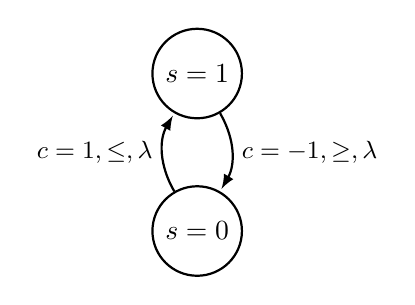
\begin{tikzpicture}[->,>=latex,shorten >=1pt,auto,node distance=2cm,
    thick,main node/.style={circle,draw}]

    \node[main node] (1) {$s=1$};
    \node[main node] (2) [below of=1] {$s=0$};

    \path[every node/.style={font=\sffamily\small}]
    (2) edge [bend left] node {$c=1, \leq, \lambda$} (1)
    (1) edge [bend left] node {$c=-1, \geq, \lambda$} (2);
  \end{tikzpicture}
  \caption{State graph for PeakSeg model.}
  \label{fig:state-graph}
\end{figure}

The algorithm recursively computes two vectors of real-valued cost
functions:
$$
\begin{array}{cccl}
  \overline C_{1}(m_1) & \cdots & \overline C_N(m_{N})& \text{ optimal cost in peak state $s=1$}\\
  \underline C_{1}(m_1) & \cdots & \underline C_N(m_{N})& \text{ optimal cost in background state $s=0$}\\
\end{array}
$$
using the update rules:
  $$\overline C_{t+1}(\mu) = \ell(\mu, z_i) + \min\{
  \overline C_t(\mu),\, 
  \underline C_t^\leq(\mu)+\lambda
\},$$
  $$\underline C_{t+1}(\mu) = \ell(\mu, z_i) + \min\{
  \underline C_t(\mu),\, 
  \overline C_t^\geq(\mu)+\lambda
\},$$
where $f^\leq(\mu) = \min_{x\leq\mu} f(x)$,\\
$f^\geq(\mu) = \min_{x\geq\mu} f(x)$.

  \begin{figure}
    \centering
    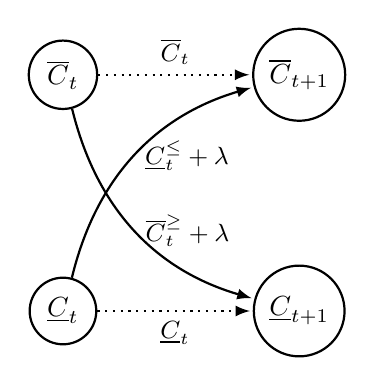
\begin{tikzpicture}[->,>=latex,shorten >=1pt,auto,node distance=3cm,
      thick,main node/.style={circle,draw}]
      \node[main node] (peak_t) {$\overline C_t$};
      \node[main node] (bkg_t) [below of=peak_t] {$\underline C_t$};
      \node[main node] (peak_t1) [right of=peak_t] {$\overline C_{t+1}$};
      \node[main node] (bkg_t1) [right of=bkg_t] {$\underline C_{t+1}$};
      \path[every node/.style={font=\small}]
      (peak_t) edge [dotted] node {$\overline C_{t}$} (peak_t1)
      (peak_t) edge [black, bend right] node [right] {$\overline C_{t}^{\geq}+\lambda$} (bkg_t1)
      (bkg_t) edge [dotted] node[midway, below] {$\underline C_{t}$} (bkg_t1)
      (bkg_t) edge [black, bend left] node[right] {$\underline C_{ t}^{\leq}+\lambda$} (peak_t1)
      ;
    \end{tikzpicture}
    \caption{Computation graph for up-down constrained model}
    \label{fig:computation-graph}
  \end{figure}


\begin{algorithm}
    \begin{algorithmic}[1]
  \STATE Input: data $\mathbf z\in\RR^N$, target peaks $P^*$.
  \STATE $\overline L,\overline p \gets \text{GFPOP}(\mathbf z, \lambda=0)$ // max peak model
  \STATE $\underline L,\underline p \gets \text{GFPOP}(\mathbf z, \lambda=\infty)$ // 0 peak model
  \STATE While $\underline p\neq P^*$ and $\overline p\neq P^*$:
  \begin{ALC@g}
    \STATE $\lambda=(\overline L-\underline L)/(\underline p-\overline p)$
    \STATE $L_{\text{new}},p_{\text{new}}\gets\text{GFPOP}(\mathbf z, \lambda)$
    \STATE If $p_{\text{new}}\in\{\underline p, \overline p\}$: return model with $\underline p$ peaks.
    \STATE If $p_{\text{new}} < P^*$: $\underline p\gets p_{\text{new}}$
    \STATE Else: $\overline p\gets p_{\text{new}}$
% > prob.i <- 3
% > fit.list$others[order(iteration)][, list(target.peaks=prob$peaks, iteration, under, over, penalty, peaks, total.cost)]
%    target.peaks iteration under over    penalty peaks total.cost
% 1:           33         1    NA   NA     0.0000  7487 -201361.96
% 2:           33         1    NA   NA        Inf     0  920923.98
% 3:           33         2     0 7487   149.8979   753  -24385.02
% 4:           33         3     0  753  1255.3904    47  153676.28
% 5:           33         4     0   47 16324.4191    10  310043.81
% 6:           33         5    10   47  4226.1495    21  214200.02
% 7:           33         6    21   47  2327.8360    33  177484.99
% > 
  \end{ALC@g}
  \STATE If $\underline p=P^*$: return model with $\underline p$ peaks.
  \STATE Else: return model with $\overline p$ peaks.
  \end{algorithmic}
\caption{\label{algo:seq-search}Sequential search for $P^*$ peaks using GFPOP.}
\end{algorithm}

Algorithm~\ref{algo:seq-search} (sequential search for $P^*$ peaks)
uses GFPOP as a sub-routine to find the optimal model with $P^*$
peaks. Its complexity is $O(N(\log N)^2)$ time, $O(N\log N)$ space,
$O(\log N)$ memory.

% \begin{leftbar}
% Note that around the \verb|{equation}| above there should be no spaces (avoided
% in the {\LaTeX} code by \verb|%| lines) so that ``normal'' spacing is used and
% not a new paragraph started.
% \end{leftbar}

% \proglang{R} provides a very flexible implementation of the general GLM
% framework in the function \fct{glm} \citep{Chambers+Hastie:1992} in the
% \pkg{stats} package. Its most important arguments are
% \begin{Code}
% glm(formula, data, subset, na.action, weights, offset,
%   family = gaussian, start = NULL, control = glm.control(...),
%   model = TRUE, y = TRUE, x = FALSE, ...)
% \end{Code}
% where \code{formula} plus \code{data} is the now standard way of specifying
% regression relationships in \proglang{R}/\proglang{S} introduced in
% \cite{Chambers+Hastie:1992}. The remaining arguments in the first line
% (\code{subset}, \code{na.action}, \code{weights}, and \code{offset}) are also
% standard  for setting up formula-based regression models in
% \proglang{R}/\proglang{S}. The arguments in the second line control aspects
% specific to GLMs while the arguments in the last line specify which components
% are returned in the fitted model object (of class \class{glm} which inherits
% from \class{lm}). For further arguments to \fct{glm} (including alternative
% specifications of starting values) see \code{?glm}. For estimating a Poisson
% model \code{family = poisson} has to be specified.

% \begin{leftbar}
% As the synopsis above is a code listing that is not meant to be executed,
% one can use either the dedicated \verb|{Code}| environment or a simple
% \verb|{verbatim}| environment for this. Again, spaces before and after should be
% avoided.

% Finally, there might be a reference to a \verb|{table}| such as
% Table~\ref{tab:overview}. Usually, these are placed at the top of the page
% (\verb|[t!]|), centered (\verb|\centering|), with a caption below the table,
% column headers and captions in sentence style, and if possible avoiding vertical
% lines.
% \end{leftbar}

% \begin{table}[t!]
% \centering
% \begin{tabular}{lllp{7.4cm}}
% \hline
% Type           & Distribution & Method   & Description \\ \hline
% GLM            & Poisson      & ML       & Poisson regression: classical GLM,
%                                            estimated by maximum likelihood (ML) \\
%                &              & Quasi    & ``Quasi-Poisson regression'':
%                                            same mean function, estimated by
%                                            quasi-ML (QML) or equivalently
%                                            generalized estimating equations (GEE),
%                                            inference adjustment via estimated
%                                            dispersion parameter \\
%                &              & Adjusted & ``Adjusted Poisson regression'':
%                                            same mean function, estimated by
%                                            QML/GEE, inference adjustment via
%                                            sandwich covariances\\
%                & NB           & ML       & NB regression: extended GLM,
%                                            estimated by ML including additional
%                                            shape parameter \\ \hline
% Zero-augmented & Poisson      & ML       & Zero-inflated Poisson (ZIP),
%                                            hurdle Poisson \\
%                & NB           & ML       & Zero-inflated NB (ZINB),
%                                            hurdle NB \\ \hline
% \end{tabular}
% \caption{\label{tab:overview} Overview of various count regression models. The
% table is usually placed at the top of the page (\texttt{[t!]}), centered
% (\texttt{centering}), has a caption below the table, column headers and captions
% are in sentence style, and if possible vertical lines should be avoided.}
% \end{table}


%% -- Illustrations ------------------------------------------------------------

%% - Virtually all JSS manuscripts list source code along with the generated
%%   output. The style files provide dedicated environments for this.
%% - In R, the environments {Sinput} and {Soutput} - as produced by Sweave() or
%%   or knitr using the render_sweave() hook - are used (without the need to
%%   load Sweave.sty).
%% - Equivalently, {CodeInput} and {CodeOutput} can be used.
%% - The code input should use "the usual" command prompt in the respective
%%   software system.
%% - For R code, the prompt "R> " should be used with "+  " as the
%%   continuation prompt.
%% - Comments within the code chunks should be avoided - these should be made
%%   within the regular LaTeX text.

\section{Illustrations} \label{sec:illustrations}

In one data set, MACS2 detected five peaks, and our GFPOP
algorithm can be used to find a more likely model with three peaks
(Figure~\ref{fig:three-peaks}). TODO

% \begin{leftbar}
% For code input and output, the style files provide dedicated environments.
% Either the ``agnostic'' \verb|{CodeInput}| and \verb|{CodeOutput}| can be used
% or, equivalently, the environments \verb|{Sinput}| and \verb|{Soutput}| as
% produced by \fct{Sweave} or \pkg{knitr} when using the \code{render_sweave()}
% hook. Please make sure that all code is properly spaced, e.g., using
% \code{y = a + b * x} and \emph{not} \code{y=a+b*x}. Moreover, code input should
% use ``the usual'' command prompt in the respective software system. For
% \proglang{R} code, the prompt \code{"R> "} should be used with \code{"+  "} as
% the continuation prompt. Generally, comments within the code chunks should be
% avoided -- and made in the regular {\LaTeX} text instead. Finally, empty lines
% before and after code input/output should be avoided (see above).
% \end{leftbar}

\begin{figure}[t!]
\centering
\includegraphics{jss-figure-label-error}
\caption{\label{fig:label-error} Labels are used to compute an error
  rate for each peak model (blue bars), defined as the sum of false
  positive and false negative labels (rectangles with black
  outline). This H3K36me3 ChIP-seq data set has $N=1,254,751$ data to
  segment on a subset of chr12, but in the plot above we show only the
  82,233 data (grey signal) in the region around the labels (colored
  rectangles). The model with penalty=6682 results in 320 peaks, which
  is too many (three false positive labels with more than one peak
  start/end). Conversely, the model with penalty=278653 results in 33
  peaks, which is too few (only two peaks in the plotted region,
  resulting in two false negative labels on the right where there
  should be exactly one peak start/end). The range of penalties between 9586 and
  267277 results in models with between 34 and 236 peaks, and achieves
  zero label errors. }
\end{figure}

\begin{figure}[t!]
\centering
%\includegraphics{jss-figure-data-peaks}
% Created by tikzDevice version 0.12.3.1 on 2021-09-17 14:13:18
% !TEX encoding = UTF-8 Unicode
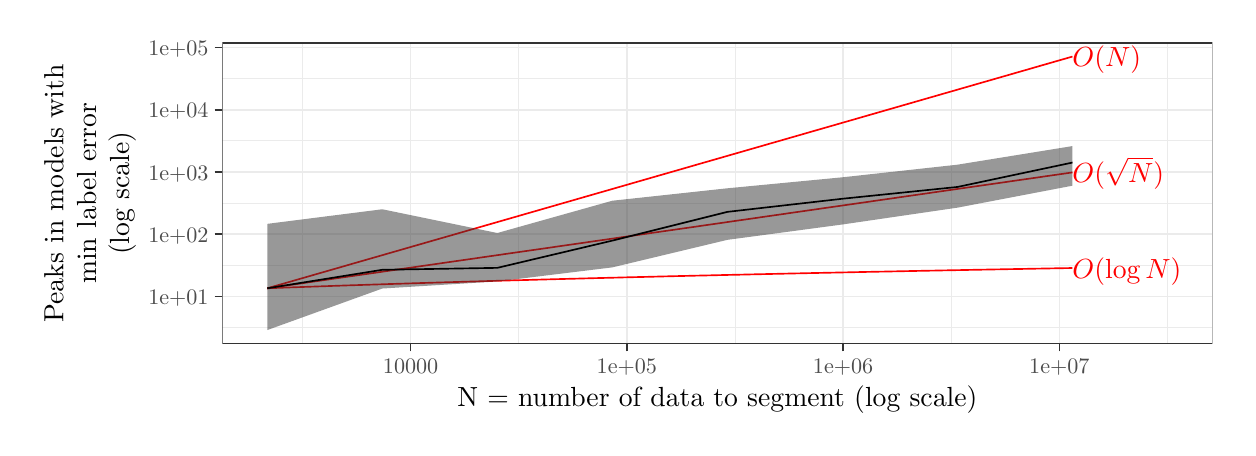
\begin{tikzpicture}[x=1pt,y=1pt]
\definecolor{fillColor}{RGB}{255,255,255}
\path[use as bounding box,fill=fillColor,fill opacity=0.00] (0,0) rectangle (433.62,144.54);
\begin{scope}
\path[clip] (  0.00,  0.00) rectangle (433.62,144.54);
\definecolor{drawColor}{RGB}{255,255,255}
\definecolor{fillColor}{RGB}{255,255,255}

\path[draw=drawColor,line width= 0.6pt,line join=round,line cap=round,fill=fillColor] (  0.00,  0.00) rectangle (433.62,144.54);
\end{scope}
\begin{scope}
\path[clip] ( 70.31, 30.33) rectangle (428.12,139.04);
\definecolor{fillColor}{RGB}{255,255,255}

\path[fill=fillColor] ( 70.31, 30.33) rectangle (428.12,139.04);
\definecolor{drawColor}{gray}{0.92}

\path[draw=drawColor,line width= 0.3pt,line join=round] ( 70.31, 36.20) --
	(428.12, 36.20);

\path[draw=drawColor,line width= 0.3pt,line join=round] ( 70.31, 58.68) --
	(428.12, 58.68);

\path[draw=drawColor,line width= 0.3pt,line join=round] ( 70.31, 81.17) --
	(428.12, 81.17);

\path[draw=drawColor,line width= 0.3pt,line join=round] ( 70.31,103.65) --
	(428.12,103.65);

\path[draw=drawColor,line width= 0.3pt,line join=round] ( 70.31,126.14) --
	(428.12,126.14);

\path[draw=drawColor,line width= 0.3pt,line join=round] ( 99.31, 30.33) --
	( 99.31,139.04);

\path[draw=drawColor,line width= 0.3pt,line join=round] (177.44, 30.33) --
	(177.44,139.04);

\path[draw=drawColor,line width= 0.3pt,line join=round] (255.58, 30.33) --
	(255.58,139.04);

\path[draw=drawColor,line width= 0.3pt,line join=round] (333.72, 30.33) --
	(333.72,139.04);

\path[draw=drawColor,line width= 0.3pt,line join=round] (411.86, 30.33) --
	(411.86,139.04);

\path[draw=drawColor,line width= 0.6pt,line join=round] ( 70.31, 47.44) --
	(428.12, 47.44);

\path[draw=drawColor,line width= 0.6pt,line join=round] ( 70.31, 69.93) --
	(428.12, 69.93);

\path[draw=drawColor,line width= 0.6pt,line join=round] ( 70.31, 92.41) --
	(428.12, 92.41);

\path[draw=drawColor,line width= 0.6pt,line join=round] ( 70.31,114.90) --
	(428.12,114.90);

\path[draw=drawColor,line width= 0.6pt,line join=round] ( 70.31,137.38) --
	(428.12,137.38);

\path[draw=drawColor,line width= 0.6pt,line join=round] (138.38, 30.33) --
	(138.38,139.04);

\path[draw=drawColor,line width= 0.6pt,line join=round] (216.51, 30.33) --
	(216.51,139.04);

\path[draw=drawColor,line width= 0.6pt,line join=round] (294.65, 30.33) --
	(294.65,139.04);

\path[draw=drawColor,line width= 0.6pt,line join=round] (372.79, 30.33) --
	(372.79,139.04);
\definecolor{drawColor}{RGB}{255,0,0}

\path[draw=drawColor,line width= 0.6pt,line join=round] ( 86.58, 50.37) --
	( 89.51, 50.48) --
	( 92.45, 50.59) --
	( 95.39, 50.70) --
	( 98.33, 50.80) --
	(101.27, 50.91) --
	(104.21, 51.01) --
	(107.15, 51.11) --
	(110.09, 51.22) --
	(113.03, 51.32) --
	(115.96, 51.42) --
	(118.90, 51.51) --
	(121.84, 51.61) --
	(124.78, 51.71) --
	(127.72, 51.80) --
	(130.66, 51.90) --
	(133.60, 51.99) --
	(136.54, 52.08) --
	(139.48, 52.18) --
	(142.42, 52.27) --
	(145.35, 52.36) --
	(148.29, 52.45) --
	(151.23, 52.54) --
	(154.17, 52.62) --
	(157.11, 52.71) --
	(160.05, 52.80) --
	(162.99, 52.88) --
	(165.93, 52.97) --
	(168.87, 53.05) --
	(171.80, 53.13) --
	(174.74, 53.22) --
	(177.68, 53.30) --
	(180.62, 53.38) --
	(183.56, 53.46) --
	(186.50, 53.54) --
	(189.44, 53.62) --
	(192.38, 53.70) --
	(195.32, 53.78) --
	(198.25, 53.85) --
	(201.19, 53.93) --
	(204.13, 54.01) --
	(207.07, 54.08) --
	(210.01, 54.16) --
	(212.95, 54.23) --
	(215.89, 54.31) --
	(218.83, 54.38) --
	(221.77, 54.45) --
	(224.71, 54.52) --
	(227.64, 54.60) --
	(230.58, 54.67) --
	(233.52, 54.74) --
	(236.46, 54.81) --
	(239.40, 54.88) --
	(242.34, 54.95) --
	(245.28, 55.01) --
	(248.22, 55.08) --
	(251.16, 55.15) --
	(254.09, 55.22) --
	(257.03, 55.28) --
	(259.97, 55.35) --
	(262.91, 55.42) --
	(265.85, 55.48) --
	(268.79, 55.55) --
	(271.73, 55.61) --
	(274.67, 55.68) --
	(277.61, 55.74) --
	(280.55, 55.80) --
	(283.48, 55.87) --
	(286.42, 55.93) --
	(289.36, 55.99) --
	(292.30, 56.05) --
	(295.24, 56.11) --
	(298.18, 56.17) --
	(301.12, 56.24) --
	(304.06, 56.30) --
	(307.00, 56.36) --
	(309.93, 56.41) --
	(312.87, 56.47) --
	(315.81, 56.53) --
	(318.75, 56.59) --
	(321.69, 56.65) --
	(324.63, 56.71) --
	(327.57, 56.76) --
	(330.51, 56.82) --
	(333.45, 56.88) --
	(336.38, 56.93) --
	(339.32, 56.99) --
	(342.26, 57.05) --
	(345.20, 57.10) --
	(348.14, 57.16) --
	(351.08, 57.21) --
	(354.02, 57.27) --
	(356.96, 57.32) --
	(359.90, 57.37) --
	(362.84, 57.43) --
	(365.77, 57.48) --
	(368.71, 57.53) --
	(371.65, 57.59) --
	(374.59, 57.64) --
	(377.53, 57.69);

\path[draw=drawColor,line width= 0.6pt,line join=round] ( 86.58, 50.37) --
	( 89.51, 50.80) --
	( 92.45, 51.22) --
	( 95.39, 51.64) --
	( 98.33, 52.06) --
	(101.27, 52.49) --
	(104.21, 52.91) --
	(107.15, 53.33) --
	(110.09, 53.76) --
	(113.03, 54.18) --
	(115.96, 54.60) --
	(118.90, 55.02) --
	(121.84, 55.45) --
	(124.78, 55.87) --
	(127.72, 56.29) --
	(130.66, 56.72) --
	(133.60, 57.14) --
	(136.54, 57.56) --
	(139.48, 57.98) --
	(142.42, 58.41) --
	(145.35, 58.83) --
	(148.29, 59.25) --
	(151.23, 59.68) --
	(154.17, 60.10) --
	(157.11, 60.52) --
	(160.05, 60.94) --
	(162.99, 61.37) --
	(165.93, 61.79) --
	(168.87, 62.21) --
	(171.80, 62.64) --
	(174.74, 63.06) --
	(177.68, 63.48) --
	(180.62, 63.90) --
	(183.56, 64.33) --
	(186.50, 64.75) --
	(189.44, 65.17) --
	(192.38, 65.60) --
	(195.32, 66.02) --
	(198.25, 66.44) --
	(201.19, 66.86) --
	(204.13, 67.29) --
	(207.07, 67.71) --
	(210.01, 68.13) --
	(212.95, 68.56) --
	(215.89, 68.98) --
	(218.83, 69.40) --
	(221.77, 69.82) --
	(224.71, 70.25) --
	(227.64, 70.67) --
	(230.58, 71.09) --
	(233.52, 71.52) --
	(236.46, 71.94) --
	(239.40, 72.36) --
	(242.34, 72.78) --
	(245.28, 73.21) --
	(248.22, 73.63) --
	(251.16, 74.05) --
	(254.09, 74.48) --
	(257.03, 74.90) --
	(259.97, 75.32) --
	(262.91, 75.74) --
	(265.85, 76.17) --
	(268.79, 76.59) --
	(271.73, 77.01) --
	(274.67, 77.44) --
	(277.61, 77.86) --
	(280.55, 78.28) --
	(283.48, 78.70) --
	(286.42, 79.13) --
	(289.36, 79.55) --
	(292.30, 79.97) --
	(295.24, 80.40) --
	(298.18, 80.82) --
	(301.12, 81.24) --
	(304.06, 81.66) --
	(307.00, 82.09) --
	(309.93, 82.51) --
	(312.87, 82.93) --
	(315.81, 83.36) --
	(318.75, 83.78) --
	(321.69, 84.20) --
	(324.63, 84.62) --
	(327.57, 85.05) --
	(330.51, 85.47) --
	(333.45, 85.89) --
	(336.38, 86.32) --
	(339.32, 86.74) --
	(342.26, 87.16) --
	(345.20, 87.58) --
	(348.14, 88.01) --
	(351.08, 88.43) --
	(354.02, 88.85) --
	(356.96, 89.28) --
	(359.90, 89.70) --
	(362.84, 90.12) --
	(365.77, 90.54) --
	(368.71, 90.97) --
	(371.65, 91.39) --
	(374.59, 91.81) --
	(377.53, 92.24);

\path[draw=drawColor,line width= 0.6pt,line join=round] ( 86.58, 50.37) --
	( 89.51, 51.22) --
	( 92.45, 52.06) --
	( 95.39, 52.91) --
	( 98.33, 53.76) --
	(101.27, 54.60) --
	(104.21, 55.45) --
	(107.15, 56.29) --
	(110.09, 57.14) --
	(113.03, 57.98) --
	(115.96, 58.83) --
	(118.90, 59.68) --
	(121.84, 60.52) --
	(124.78, 61.37) --
	(127.72, 62.21) --
	(130.66, 63.06) --
	(133.60, 63.90) --
	(136.54, 64.75) --
	(139.48, 65.60) --
	(142.42, 66.44) --
	(145.35, 67.29) --
	(148.29, 68.13) --
	(151.23, 68.98) --
	(154.17, 69.82) --
	(157.11, 70.67) --
	(160.05, 71.52) --
	(162.99, 72.36) --
	(165.93, 73.21) --
	(168.87, 74.05) --
	(171.80, 74.90) --
	(174.74, 75.74) --
	(177.68, 76.59) --
	(180.62, 77.44) --
	(183.56, 78.28) --
	(186.50, 79.13) --
	(189.44, 79.97) --
	(192.38, 80.82) --
	(195.32, 81.66) --
	(198.25, 82.51) --
	(201.19, 83.36) --
	(204.13, 84.20) --
	(207.07, 85.05) --
	(210.01, 85.89) --
	(212.95, 86.74) --
	(215.89, 87.58) --
	(218.83, 88.43) --
	(221.77, 89.28) --
	(224.71, 90.12) --
	(227.64, 90.97) --
	(230.58, 91.81) --
	(233.52, 92.66) --
	(236.46, 93.50) --
	(239.40, 94.35) --
	(242.34, 95.20) --
	(245.28, 96.04) --
	(248.22, 96.89) --
	(251.16, 97.73) --
	(254.09, 98.58) --
	(257.03, 99.42) --
	(259.97,100.27) --
	(262.91,101.12) --
	(265.85,101.96) --
	(268.79,102.81) --
	(271.73,103.65) --
	(274.67,104.50) --
	(277.61,105.34) --
	(280.55,106.19) --
	(283.48,107.04) --
	(286.42,107.88) --
	(289.36,108.73) --
	(292.30,109.57) --
	(295.24,110.42) --
	(298.18,111.26) --
	(301.12,112.11) --
	(304.06,112.96) --
	(307.00,113.80) --
	(309.93,114.65) --
	(312.87,115.49) --
	(315.81,116.34) --
	(318.75,117.18) --
	(321.69,118.03) --
	(324.63,118.88) --
	(327.57,119.72) --
	(330.51,120.57) --
	(333.45,121.41) --
	(336.38,122.26) --
	(339.32,123.10) --
	(342.26,123.95) --
	(345.20,124.80) --
	(348.14,125.64) --
	(351.08,126.49) --
	(354.02,127.33) --
	(356.96,128.18) --
	(359.90,129.02) --
	(362.84,129.87) --
	(365.77,130.72) --
	(368.71,131.56) --
	(371.65,132.41) --
	(374.59,133.25) --
	(377.53,134.10);

\node[text=drawColor,anchor=base west,inner sep=0pt, outer sep=0pt, scale=  1.00] at (377.53,130.39) {$O(N)$};

\node[text=drawColor,anchor=base west,inner sep=0pt, outer sep=0pt, scale=  1.00] at (377.53, 53.98) {$O(\log N)$};

\node[text=drawColor,anchor=base west,inner sep=0pt, outer sep=0pt, scale=  1.00] at (377.53, 88.53) {$O(\sqrt N)$};
\definecolor{fillColor}{RGB}{51,51,51}

\path[fill=fillColor,fill opacity=0.50] ( 86.58, 73.65) --
	(128.14, 78.92) --
	(169.71, 70.34) --
	(211.27, 82.01) --
	(252.84, 86.50) --
	(294.40, 90.47) --
	(335.97, 95.03) --
	(377.53,101.75) --
	(377.53, 87.44) --
	(335.97, 79.50) --
	(294.40, 73.42) --
	(252.84, 67.87) --
	(211.27, 57.92) --
	(169.71, 52.84) --
	(128.14, 50.28) --
	( 86.58, 35.27) --
	cycle;

\path[] ( 86.58, 73.65) --
	(128.14, 78.92) --
	(169.71, 70.34) --
	(211.27, 82.01) --
	(252.84, 86.50) --
	(294.40, 90.47) --
	(335.97, 95.03) --
	(377.53,101.75);

\path[] (377.53, 87.44) --
	(335.97, 79.50) --
	(294.40, 73.42) --
	(252.84, 67.87) --
	(211.27, 57.92) --
	(169.71, 52.84) --
	(128.14, 50.28) --
	( 86.58, 35.27);
\definecolor{drawColor}{RGB}{0,0,0}

\path[draw=drawColor,line width= 0.6pt,line join=round] ( 86.58, 50.37) --
	(128.14, 57.05) --
	(169.71, 57.75) --
	(211.27, 67.59) --
	(252.84, 77.98) --
	(294.40, 82.72) --
	(335.97, 86.98) --
	(377.53, 95.80);
\definecolor{drawColor}{gray}{0.20}

\path[draw=drawColor,line width= 0.6pt,line join=round,line cap=round] ( 70.31, 30.33) rectangle (428.12,139.04);
\end{scope}
\begin{scope}
\path[clip] (  0.00,  0.00) rectangle (433.62,144.54);
\definecolor{drawColor}{gray}{0.30}

\node[text=drawColor,anchor=base east,inner sep=0pt, outer sep=0pt, scale=  0.80] at ( 65.36, 44.49) {1e+01};

\node[text=drawColor,anchor=base east,inner sep=0pt, outer sep=0pt, scale=  0.80] at ( 65.36, 66.97) {1e+02};

\node[text=drawColor,anchor=base east,inner sep=0pt, outer sep=0pt, scale=  0.80] at ( 65.36, 89.46) {1e+03};

\node[text=drawColor,anchor=base east,inner sep=0pt, outer sep=0pt, scale=  0.80] at ( 65.36,111.94) {1e+04};

\node[text=drawColor,anchor=base east,inner sep=0pt, outer sep=0pt, scale=  0.80] at ( 65.36,134.43) {1e+05};
\end{scope}
\begin{scope}
\path[clip] (  0.00,  0.00) rectangle (433.62,144.54);
\definecolor{drawColor}{gray}{0.20}

\path[draw=drawColor,line width= 0.6pt,line join=round] ( 67.56, 47.44) --
	( 70.31, 47.44);

\path[draw=drawColor,line width= 0.6pt,line join=round] ( 67.56, 69.93) --
	( 70.31, 69.93);

\path[draw=drawColor,line width= 0.6pt,line join=round] ( 67.56, 92.41) --
	( 70.31, 92.41);

\path[draw=drawColor,line width= 0.6pt,line join=round] ( 67.56,114.90) --
	( 70.31,114.90);

\path[draw=drawColor,line width= 0.6pt,line join=round] ( 67.56,137.38) --
	( 70.31,137.38);
\end{scope}
\begin{scope}
\path[clip] (  0.00,  0.00) rectangle (433.62,144.54);
\definecolor{drawColor}{gray}{0.20}

\path[draw=drawColor,line width= 0.6pt,line join=round] (138.38, 27.58) --
	(138.38, 30.33);

\path[draw=drawColor,line width= 0.6pt,line join=round] (216.51, 27.58) --
	(216.51, 30.33);

\path[draw=drawColor,line width= 0.6pt,line join=round] (294.65, 27.58) --
	(294.65, 30.33);

\path[draw=drawColor,line width= 0.6pt,line join=round] (372.79, 27.58) --
	(372.79, 30.33);
\end{scope}
\begin{scope}
\path[clip] (  0.00,  0.00) rectangle (433.62,144.54);
\definecolor{drawColor}{gray}{0.30}

\node[text=drawColor,anchor=base,inner sep=0pt, outer sep=0pt, scale=  0.80] at (138.38, 19.46) {10000};

\node[text=drawColor,anchor=base,inner sep=0pt, outer sep=0pt, scale=  0.80] at (216.51, 19.46) {1e+05};

\node[text=drawColor,anchor=base,inner sep=0pt, outer sep=0pt, scale=  0.80] at (294.65, 19.46) {1e+06};

\node[text=drawColor,anchor=base,inner sep=0pt, outer sep=0pt, scale=  0.80] at (372.79, 19.46) {1e+07};
\end{scope}
\begin{scope}
\path[clip] (  0.00,  0.00) rectangle (433.62,144.54);
\definecolor{drawColor}{RGB}{0,0,0}

\node[text=drawColor,anchor=base,inner sep=0pt, outer sep=0pt, scale=  1.00] at (249.22,  7.62) {N = number of data to segment (log scale)};
\end{scope}
\begin{scope}
\path[clip] (  0.00,  0.00) rectangle (433.62,144.54);
\definecolor{drawColor}{RGB}{0,0,0}

\node[text=drawColor,rotate= 90.00,anchor=base,inner sep=0pt, outer sep=0pt, scale=  1.00] at ( 12.89, 84.68) {Peaks in models with};

\node[text=drawColor,rotate= 90.00,anchor=base,inner sep=0pt, outer sep=0pt, scale=  1.00] at ( 24.77, 84.68) {min label error};

\node[text=drawColor,rotate= 90.00,anchor=base,inner sep=0pt, outer sep=0pt, scale=  1.00] at ( 36.65, 84.68) {(log scale)};
\end{scope}
\end{tikzpicture}

\caption{\label{fig:data-peaks} The model with minimal label
  errors has $O(\sqrt{N})$ peaks in a data set of size $N$. For each data set we
  computed peak models with minimal label errors (see
  Figure~\ref{fig:label-error}); we then plot the number of peaks in
  minimal error models as a function of data set size $N$. Black median line
  and grey quartile band computed over several data sets of a given size
  $N$; asymptotic reference lines shown in red.}
\end{figure}
  
% \begin{figure}[t!] 
% \centering
% \includegraphics{jss-figure-more-likely-models-one-peak}
% \caption{\label{fig:one-peak} Default peak model from the baseline
%   MACS2 algorithm (top) and the optimal peak model computed using the
%   proposed PeakSegFPOP algorithm (bottom).}
% \end{figure}

% \begin{figure}[t!]
% \centering
% \includegraphics{jss-figure-target-intervals-models-penalty}
% \caption{\label{fig:target-intervals-models-penalty} The PeakSegFPOP
%   algorithm was used to compute optimal models for six of the largest
%   problems (panels from left to right) for a variety of penalty
%   parameters (x-axis). Y-axes show empirical measurements of cost
%   function pieces (intervals, top panel), timings (minutes, middle
%   panel), and disk usage (gigabytes, bottom panel).}
% \end{figure}

\begin{figure}[t!]
\centering
\begin{minipage}{3in}
  \includegraphics{jss-figure-disk-memory-compare-speed}
\end{minipage} 
\begin{minipage}{3in}
  \includegraphics{jss-figure-disk-memory-compare-speed-penalty}
\end{minipage}
\caption{\label{fig:disk-memory-compare-speed} The disk-based storage
  method is only a constant factor slower than the memory-based
  method. We benchmarked both methods on several small data sets
  ($N\leq 462,890$) for which optimal models could be computed using
  1GB of storage. \textbf{Left:} computation time is empirically
  $O(N\log N)$ for both storage methods, but the disk-based method is
  slower by a constant factor. Median line and quartile band computed
  over several penalty values for a given data set; black vertical
  line segment highlights the data set with $N=106,569$ used in the
  right panel. \textbf{Right:} computation time increases with penalty
  value $\lambda$ for both methods, with the disk-based method slower
  by a constant factor.}
\end{figure}

% \begin{figure}[t!]
% \centering
% \includegraphics{jss-figure-target-intervals-models-all}
% \caption{\label{fig:target-intervals-models-all} The PeakSegFPOP algorithm
%   was used on the large data sets in the
%   benchmark. Data sizes range from $N=10^2$ to $10^7$ weighted data to
%   segment (x-axis); disk usage (top panel) and computation time
%   (bottom panel) are log-linear $O(N \log N)$.}
% \end{figure}
 
\begin{figure}[t!]
\centering
\begin{minipage}{3in}
  \includegraphics{jss-figure-target-intervals-models}
\end{minipage} 
\begin{minipage}{3in}
  \includegraphics{jss-figure-target-intervals-models-computation}
\end{minipage}
\caption{\label{fig:target-intervals-models-all} In our empirical
  tests, the computational requirements of the GFPOP algorithm
  were log-linear $O(N \log N)$ in the number of data points $N$ to
  segment. \textbf{Left:} we analyzed the number of intervals $I$
  (candidate changepoints) stored in the $C_t(\mu)$ cost functions,
  because the total time/space complexity is $O(NI)$. We observed
  empirically that the mean number of intervals $I=O(\log N)$ (red
  curve). Even the maximum number of intervals (blue curve) is much
  less than $N$. \textbf{Right:} storage on disk (top panel) and
  computation time (bottom panel) are empirically $O(N \log N)$. Error
  bands show median and 5\%/95\% quantiles over several data sets of a
  given size $N$; black dots and text show computational requirements
  for the most extreme data sets.}
\end{figure}

\begin{figure}[t!]
\centering
\begin{minipage}{3in}
  %\includegraphics{jss-figure-evaluations}
  % Created by tikzDevice version 0.12.3.1 on 2021-08-27 11:08:28
% !TEX encoding = UTF-8 Unicode
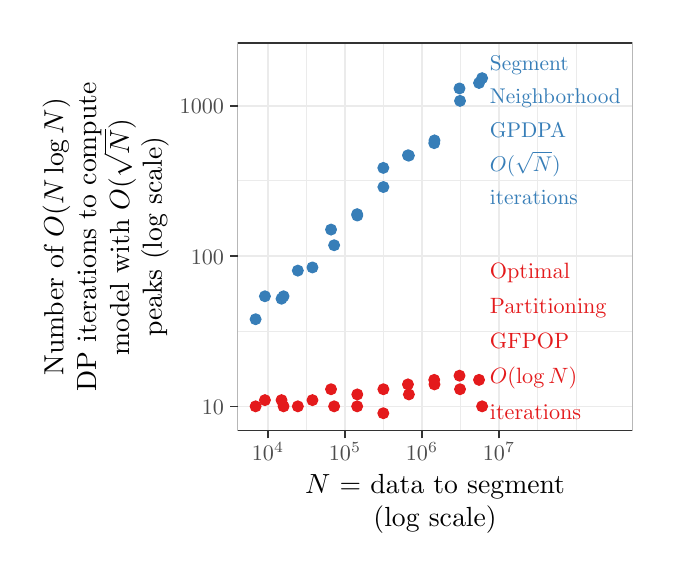
\begin{tikzpicture}[x=1pt,y=1pt]
\definecolor{fillColor}{RGB}{255,255,255}
\path[use as bounding box,fill=fillColor,fill opacity=0.00] (0,0) rectangle (224.04,187.90);
\begin{scope}
\path[clip] (  0.00,  0.00) rectangle (224.04,187.90);
\definecolor{drawColor}{RGB}{255,255,255}
\definecolor{fillColor}{RGB}{255,255,255}

\path[draw=drawColor,line width= 0.6pt,line join=round,line cap=round,fill=fillColor] (  0.00,  0.00) rectangle (224.04,187.90);
\end{scope}
\begin{scope}
\path[clip] ( 75.88, 42.21) rectangle (218.54,182.40);
\definecolor{fillColor}{RGB}{255,255,255}

\path[fill=fillColor] ( 75.88, 42.21) rectangle (218.54,182.40);
\definecolor{drawColor}{gray}{0.92}

\path[draw=drawColor,line width= 0.3pt,line join=round] ( 75.88, 78.22) --
	(218.54, 78.22);

\path[draw=drawColor,line width= 0.3pt,line join=round] ( 75.88,132.53) --
	(218.54,132.53);

\path[draw=drawColor,line width= 0.3pt,line join=round] (100.72, 42.21) --
	(100.72,182.40);

\path[draw=drawColor,line width= 0.3pt,line join=round] (128.56, 42.21) --
	(128.56,182.40);

\path[draw=drawColor,line width= 0.3pt,line join=round] (156.39, 42.21) --
	(156.39,182.40);

\path[draw=drawColor,line width= 0.3pt,line join=round] (184.22, 42.21) --
	(184.22,182.40);

\path[draw=drawColor,line width= 0.3pt,line join=round] (198.14, 42.21) --
	(198.14,182.40);

\path[draw=drawColor,line width= 0.6pt,line join=round] ( 75.88, 51.07) --
	(218.54, 51.07);

\path[draw=drawColor,line width= 0.6pt,line join=round] ( 75.88,105.37) --
	(218.54,105.37);

\path[draw=drawColor,line width= 0.6pt,line join=round] ( 75.88,159.68) --
	(218.54,159.68);

\path[draw=drawColor,line width= 0.6pt,line join=round] ( 86.81, 42.21) --
	( 86.81,182.40);

\path[draw=drawColor,line width= 0.6pt,line join=round] (114.64, 42.21) --
	(114.64,182.40);

\path[draw=drawColor,line width= 0.6pt,line join=round] (142.47, 42.21) --
	(142.47,182.40);

\path[draw=drawColor,line width= 0.6pt,line join=round] (170.30, 42.21) --
	(170.30,182.40);
\definecolor{drawColor}{RGB}{55,126,184}
\definecolor{fillColor}{RGB}{55,126,184}

\path[draw=drawColor,line width= 0.4pt,line join=round,line cap=round,fill=fillColor] ( 82.36, 82.55) circle (  1.96);

\path[draw=drawColor,line width= 0.4pt,line join=round,line cap=round,fill=fillColor] ( 85.73, 90.84) circle (  1.96);

\path[draw=drawColor,line width= 0.4pt,line join=round,line cap=round,fill=fillColor] ( 91.73, 89.95) circle (  1.96);

\path[draw=drawColor,line width= 0.4pt,line join=round,line cap=round,fill=fillColor] ( 92.46, 90.84) circle (  1.96);

\path[draw=drawColor,line width= 0.4pt,line join=round,line cap=round,fill=fillColor] ( 97.62,100.11) circle (  1.96);

\path[draw=drawColor,line width= 0.4pt,line join=round,line cap=round,fill=fillColor] (102.90,101.26) circle (  1.96);

\path[draw=drawColor,line width= 0.4pt,line join=round,line cap=round,fill=fillColor] (109.62,114.94) circle (  1.96);

\path[draw=drawColor,line width= 0.4pt,line join=round,line cap=round,fill=fillColor] (110.74,109.28) circle (  1.96);

\path[draw=drawColor,line width= 0.4pt,line join=round,line cap=round,fill=fillColor] (119.06,120.51) circle (  1.96);

\path[draw=drawColor,line width= 0.4pt,line join=round,line cap=round,fill=fillColor] (119.11,120.01) circle (  1.96);

\path[draw=drawColor,line width= 0.4pt,line join=round,line cap=round,fill=fillColor] (128.51,137.23) circle (  1.96);

\path[draw=drawColor,line width= 0.4pt,line join=round,line cap=round,fill=fillColor] (128.54,130.32) circle (  1.96);

\path[draw=drawColor,line width= 0.4pt,line join=round,line cap=round,fill=fillColor] (137.41,141.77) circle (  1.96);

\path[draw=drawColor,line width= 0.4pt,line join=round,line cap=round,fill=fillColor] (137.75,141.67) circle (  1.96);

\path[draw=drawColor,line width= 0.4pt,line join=round,line cap=round,fill=fillColor] (146.90,146.17) circle (  1.96);

\path[draw=drawColor,line width= 0.4pt,line join=round,line cap=round,fill=fillColor] (147.00,147.16) circle (  1.96);

\path[draw=drawColor,line width= 0.4pt,line join=round,line cap=round,fill=fillColor] (156.04,165.94) circle (  1.96);

\path[draw=drawColor,line width= 0.4pt,line join=round,line cap=round,fill=fillColor] (156.23,161.45) circle (  1.96);

\path[draw=drawColor,line width= 0.4pt,line join=round,line cap=round,fill=fillColor] (163.10,167.92) circle (  1.96);

\path[draw=drawColor,line width= 0.4pt,line join=round,line cap=round,fill=fillColor] (164.21,169.65) circle (  1.96);
\definecolor{drawColor}{RGB}{228,26,28}
\definecolor{fillColor}{RGB}{228,26,28}

\path[draw=drawColor,line width= 0.4pt,line join=round,line cap=round,fill=fillColor] ( 82.36, 51.07) circle (  1.96);

\path[draw=drawColor,line width= 0.4pt,line join=round,line cap=round,fill=fillColor] ( 85.73, 53.31) circle (  1.96);

\path[draw=drawColor,line width= 0.4pt,line join=round,line cap=round,fill=fillColor] ( 91.73, 53.31) circle (  1.96);

\path[draw=drawColor,line width= 0.4pt,line join=round,line cap=round,fill=fillColor] ( 92.46, 51.07) circle (  1.96);

\path[draw=drawColor,line width= 0.4pt,line join=round,line cap=round,fill=fillColor] ( 97.62, 51.07) circle (  1.96);

\path[draw=drawColor,line width= 0.4pt,line join=round,line cap=round,fill=fillColor] (102.90, 53.31) circle (  1.96);

\path[draw=drawColor,line width= 0.4pt,line join=round,line cap=round,fill=fillColor] (109.62, 57.25) circle (  1.96);

\path[draw=drawColor,line width= 0.4pt,line join=round,line cap=round,fill=fillColor] (110.74, 51.07) circle (  1.96);

\path[draw=drawColor,line width= 0.4pt,line join=round,line cap=round,fill=fillColor] (119.06, 51.07) circle (  1.96);

\path[draw=drawColor,line width= 0.4pt,line join=round,line cap=round,fill=fillColor] (119.11, 55.37) circle (  1.96);

\path[draw=drawColor,line width= 0.4pt,line join=round,line cap=round,fill=fillColor] (128.51, 48.58) circle (  1.96);

\path[draw=drawColor,line width= 0.4pt,line join=round,line cap=round,fill=fillColor] (128.54, 57.25) circle (  1.96);

\path[draw=drawColor,line width= 0.4pt,line join=round,line cap=round,fill=fillColor] (137.41, 59.00) circle (  1.96);

\path[draw=drawColor,line width= 0.4pt,line join=round,line cap=round,fill=fillColor] (137.75, 55.37) circle (  1.96);

\path[draw=drawColor,line width= 0.4pt,line join=round,line cap=round,fill=fillColor] (146.90, 60.63) circle (  1.96);

\path[draw=drawColor,line width= 0.4pt,line join=round,line cap=round,fill=fillColor] (147.00, 59.00) circle (  1.96);

\path[draw=drawColor,line width= 0.4pt,line join=round,line cap=round,fill=fillColor] (156.04, 62.15) circle (  1.96);

\path[draw=drawColor,line width= 0.4pt,line join=round,line cap=round,fill=fillColor] (156.23, 57.25) circle (  1.96);

\path[draw=drawColor,line width= 0.4pt,line join=round,line cap=round,fill=fillColor] (163.10, 60.63) circle (  1.96);

\path[draw=drawColor,line width= 0.4pt,line join=round,line cap=round,fill=fillColor] (164.21, 51.07) circle (  1.96);
\end{scope}
\begin{scope}
\path[clip] ( 75.88, 42.21) rectangle (218.54,182.40);
\definecolor{drawColor}{RGB}{228,26,28}

\node[text=drawColor,anchor=base west,inner sep=0pt, outer sep=0pt, scale=  0.80] at (167.05, 97.16) {Optimal};

\node[text=drawColor,anchor=base west,inner sep=0pt, outer sep=0pt, scale=  0.80] at (167.05, 84.49) {Partitioning};

\node[text=drawColor,anchor=base west,inner sep=0pt, outer sep=0pt, scale=  0.80] at (167.05, 71.82) {GFPOP};

\node[text=drawColor,anchor=base west,inner sep=0pt, outer sep=0pt, scale=  0.80] at (167.05, 59.15) {$O(\log N)$};

\node[text=drawColor,anchor=base west,inner sep=0pt, outer sep=0pt, scale=  0.80] at (167.05, 46.48) {iterations};
\definecolor{drawColor}{RGB}{55,126,184}

\node[text=drawColor,anchor=base west,inner sep=0pt, outer sep=0pt, scale=  0.77] at (167.05,172.47) {Segment};

\node[text=drawColor,anchor=base west,inner sep=0pt, outer sep=0pt, scale=  0.77] at (167.05,160.33) {Neighborhood};

\node[text=drawColor,anchor=base west,inner sep=0pt, outer sep=0pt, scale=  0.77] at (167.05,148.19) {GPDPA};

\node[text=drawColor,anchor=base west,inner sep=0pt, outer sep=0pt, scale=  0.77] at (167.05,136.06) {$O(\sqrt N)$};

\node[text=drawColor,anchor=base west,inner sep=0pt, outer sep=0pt, scale=  0.77] at (167.05,123.92) {iterations};
\definecolor{drawColor}{gray}{0.20}

\path[draw=drawColor,line width= 0.6pt,line join=round,line cap=round] ( 75.88, 42.21) rectangle (218.54,182.40);
\end{scope}
\begin{scope}
\path[clip] (  0.00,  0.00) rectangle (224.04,187.90);
\definecolor{drawColor}{gray}{0.30}

\node[text=drawColor,anchor=base east,inner sep=0pt, outer sep=0pt, scale=  0.80] at ( 70.93, 48.11) {10};

\node[text=drawColor,anchor=base east,inner sep=0pt, outer sep=0pt, scale=  0.80] at ( 70.93,102.42) {100};

\node[text=drawColor,anchor=base east,inner sep=0pt, outer sep=0pt, scale=  0.80] at ( 70.93,156.72) {1000};
\end{scope}
\begin{scope}
\path[clip] (  0.00,  0.00) rectangle (224.04,187.90);
\definecolor{drawColor}{gray}{0.20}

\path[draw=drawColor,line width= 0.6pt,line join=round] ( 73.13, 51.07) --
	( 75.88, 51.07);

\path[draw=drawColor,line width= 0.6pt,line join=round] ( 73.13,105.37) --
	( 75.88,105.37);

\path[draw=drawColor,line width= 0.6pt,line join=round] ( 73.13,159.68) --
	( 75.88,159.68);
\end{scope}
\begin{scope}
\path[clip] (  0.00,  0.00) rectangle (224.04,187.90);
\definecolor{drawColor}{gray}{0.20}

\path[draw=drawColor,line width= 0.6pt,line join=round] ( 86.81, 39.46) --
	( 86.81, 42.21);

\path[draw=drawColor,line width= 0.6pt,line join=round] (114.64, 39.46) --
	(114.64, 42.21);

\path[draw=drawColor,line width= 0.6pt,line join=round] (142.47, 39.46) --
	(142.47, 42.21);

\path[draw=drawColor,line width= 0.6pt,line join=round] (170.30, 39.46) --
	(170.30, 42.21);
\end{scope}
\begin{scope}
\path[clip] (  0.00,  0.00) rectangle (224.04,187.90);
\definecolor{drawColor}{gray}{0.30}

\node[text=drawColor,anchor=base,inner sep=0pt, outer sep=0pt, scale=  0.80] at ( 86.81, 31.34) {$10^4$};

\node[text=drawColor,anchor=base,inner sep=0pt, outer sep=0pt, scale=  0.80] at (114.64, 31.34) {$10^5$};

\node[text=drawColor,anchor=base,inner sep=0pt, outer sep=0pt, scale=  0.80] at (142.47, 31.34) {$10^6$};

\node[text=drawColor,anchor=base,inner sep=0pt, outer sep=0pt, scale=  0.80] at (170.30, 31.34) {$10^7$};
\end{scope}
\begin{scope}
\path[clip] (  0.00,  0.00) rectangle (224.04,187.90);
\definecolor{drawColor}{RGB}{0,0,0}

\node[text=drawColor,anchor=base,inner sep=0pt, outer sep=0pt, scale=  1.00] at (147.21, 19.50) {$N$ = data to segment};

\node[text=drawColor,anchor=base,inner sep=0pt, outer sep=0pt, scale=  1.00] at (147.21,  7.62) {(log scale)};
\end{scope}
\begin{scope}
\path[clip] (  0.00,  0.00) rectangle (224.04,187.90);
\definecolor{drawColor}{RGB}{0,0,0}

\node[text=drawColor,rotate= 90.00,anchor=base,inner sep=0pt, outer sep=0pt, scale=  1.00] at ( 12.89,112.30) {Number of $O(N \log N)$};

\node[text=drawColor,rotate= 90.00,anchor=base,inner sep=0pt, outer sep=0pt, scale=  1.00] at ( 24.77,112.30) {DP iterations to compute};

\node[text=drawColor,rotate= 90.00,anchor=base,inner sep=0pt, outer sep=0pt, scale=  1.00] at ( 36.65,112.30) {model with $O(\sqrt N)$};

\node[text=drawColor,rotate= 90.00,anchor=base,inner sep=0pt, outer sep=0pt, scale=  1.00] at ( 48.53,112.30) {peaks (log scale)};
\end{scope}
\end{tikzpicture}

\end{minipage} 
\begin{minipage}{3in} 
  %\includegraphics{jss-figure-evaluations-computation}
  % Created by tikzDevice version 0.12.3.1 on 2021-08-27 11:08:28
% !TEX encoding = UTF-8 Unicode
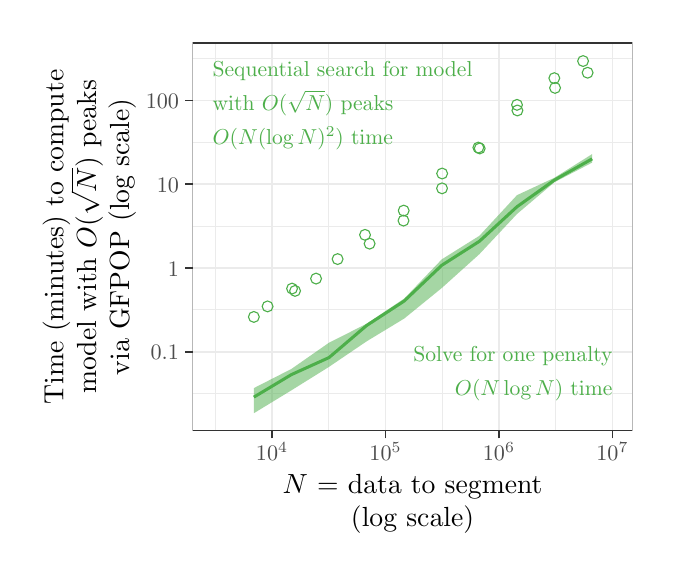
\begin{tikzpicture}[x=1pt,y=1pt]
\definecolor{fillColor}{RGB}{255,255,255}
\path[use as bounding box,fill=fillColor,fill opacity=0.00] (0,0) rectangle (224.04,187.90);
\begin{scope}
\path[clip] (  0.00,  0.00) rectangle (224.04,187.90);
\definecolor{drawColor}{RGB}{255,255,255}
\definecolor{fillColor}{RGB}{255,255,255}

\path[draw=drawColor,line width= 0.6pt,line join=round,line cap=round,fill=fillColor] ( -0.00,  0.00) rectangle (224.04,187.90);
\end{scope}
\begin{scope}
\path[clip] ( 59.62, 42.21) rectangle (218.54,182.40);
\definecolor{fillColor}{RGB}{255,255,255}

\path[fill=fillColor] ( 59.62, 42.21) rectangle (218.54,182.40);
\definecolor{drawColor}{gray}{0.92}

\path[draw=drawColor,line width= 0.3pt,line join=round] ( 59.62, 55.66) --
	(218.54, 55.66);

\path[draw=drawColor,line width= 0.3pt,line join=round] ( 59.62, 85.93) --
	(218.54, 85.93);

\path[draw=drawColor,line width= 0.3pt,line join=round] ( 59.62,116.19) --
	(218.54,116.19);

\path[draw=drawColor,line width= 0.3pt,line join=round] ( 59.62,146.46) --
	(218.54,146.46);

\path[draw=drawColor,line width= 0.3pt,line join=round] ( 59.62,176.72) --
	(218.54,176.72);

\path[draw=drawColor,line width= 0.3pt,line join=round] ( 67.78, 42.21) --
	( 67.78,182.40);

\path[draw=drawColor,line width= 0.3pt,line join=round] (108.79, 42.21) --
	(108.79,182.40);

\path[draw=drawColor,line width= 0.3pt,line join=round] (149.80, 42.21) --
	(149.80,182.40);

\path[draw=drawColor,line width= 0.3pt,line join=round] (190.81, 42.21) --
	(190.81,182.40);

\path[draw=drawColor,line width= 0.6pt,line join=round] ( 59.62, 70.79) --
	(218.54, 70.79);

\path[draw=drawColor,line width= 0.6pt,line join=round] ( 59.62,101.06) --
	(218.54,101.06);

\path[draw=drawColor,line width= 0.6pt,line join=round] ( 59.62,131.32) --
	(218.54,131.32);

\path[draw=drawColor,line width= 0.6pt,line join=round] ( 59.62,161.59) --
	(218.54,161.59);

\path[draw=drawColor,line width= 0.6pt,line join=round] ( 88.28, 42.21) --
	( 88.28,182.40);

\path[draw=drawColor,line width= 0.6pt,line join=round] (129.29, 42.21) --
	(129.29,182.40);

\path[draw=drawColor,line width= 0.6pt,line join=round] (170.30, 42.21) --
	(170.30,182.40);

\path[draw=drawColor,line width= 0.6pt,line join=round] (211.31, 42.21) --
	(211.31,182.40);
\definecolor{drawColor}{RGB}{77,175,74}

\node[text=drawColor,anchor=base west,inner sep=0pt, outer sep=0pt, scale=  0.78] at ( 66.84,170.29) {Sequential search for model};

\node[text=drawColor,anchor=base west,inner sep=0pt, outer sep=0pt, scale=  0.78] at ( 66.84,158.00) {with $O(\sqrt N)$ peaks};

\node[text=drawColor,anchor=base west,inner sep=0pt, outer sep=0pt, scale=  0.78] at ( 66.84,145.71) {$O(N(\log N)^2)$ time};

\node[text=drawColor,anchor=base east,inner sep=0pt, outer sep=0pt, scale=  0.78] at (211.31, 67.26) {Solve for one penalty};

\node[text=drawColor,anchor=base east,inner sep=0pt, outer sep=0pt, scale=  0.78] at (211.31, 54.97) {$O(N \log N)$ time};
\definecolor{fillColor}{RGB}{77,175,74}

\path[fill=fillColor,fill opacity=0.50] ( 81.73, 57.66) --
	( 95.31, 64.59) --
	(108.89, 74.06) --
	(122.47, 80.91) --
	(136.06, 90.01) --
	(149.64,104.19) --
	(163.22,112.69) --
	(176.80,127.37) --
	(190.38,133.69) --
	(203.97,142.22) --
	(203.97,139.13) --
	(190.38,132.07) --
	(176.80,120.56) --
	(163.22,106.05) --
	(149.64, 93.83) --
	(136.06, 82.79) --
	(122.47, 74.55) --
	(108.89, 65.34) --
	( 95.31, 56.86) --
	( 81.73, 48.58) --
	cycle;

\path[] ( 81.73, 57.66) --
	( 95.31, 64.59) --
	(108.89, 74.06) --
	(122.47, 80.91) --
	(136.06, 90.01) --
	(149.64,104.19) --
	(163.22,112.69) --
	(176.80,127.37) --
	(190.38,133.69) --
	(203.97,142.22);

\path[] (203.97,139.13) --
	(190.38,132.07) --
	(176.80,120.56) --
	(163.22,106.05) --
	(149.64, 93.83) --
	(136.06, 82.79) --
	(122.47, 74.55) --
	(108.89, 65.34) --
	( 95.31, 56.86) --
	( 81.73, 48.58);

\path[draw=drawColor,line width= 1.1pt,line join=round] ( 81.73, 54.40) --
	( 95.31, 62.54) --
	(108.89, 68.69) --
	(122.47, 80.27) --
	(136.06, 89.12) --
	(149.64,102.04) --
	(163.22,110.70) --
	(176.80,123.18) --
	(190.38,132.86) --
	(203.97,140.50);

\path[draw=drawColor,line width= 0.4pt,line join=round,line cap=round] ( 81.73, 83.38) circle (  1.96);

\path[draw=drawColor,line width= 0.4pt,line join=round,line cap=round] ( 86.69, 87.18) circle (  1.96);

\path[draw=drawColor,line width= 0.4pt,line join=round,line cap=round] ( 95.53, 93.62) circle (  1.96);

\path[draw=drawColor,line width= 0.4pt,line join=round,line cap=round] ( 96.62, 92.78) circle (  1.96);

\path[draw=drawColor,line width= 0.4pt,line join=round,line cap=round] (104.21, 97.23) circle (  1.96);

\path[draw=drawColor,line width= 0.4pt,line join=round,line cap=round] (111.99,104.28) circle (  1.96);

\path[draw=drawColor,line width= 0.4pt,line join=round,line cap=round] (121.90,113.04) circle (  1.96);

\path[draw=drawColor,line width= 0.4pt,line join=round,line cap=round] (123.55,109.85) circle (  1.96);

\path[draw=drawColor,line width= 0.4pt,line join=round,line cap=round] (135.80,118.18) circle (  1.96);

\path[draw=drawColor,line width= 0.4pt,line join=round,line cap=round] (135.87,121.80) circle (  1.96);

\path[draw=drawColor,line width= 0.4pt,line join=round,line cap=round] (149.73,129.84) circle (  1.96);

\path[draw=drawColor,line width= 0.4pt,line join=round,line cap=round] (149.77,135.20) circle (  1.96);

\path[draw=drawColor,line width= 0.4pt,line join=round,line cap=round] (162.85,144.58) circle (  1.96);

\path[draw=drawColor,line width= 0.4pt,line join=round,line cap=round] (163.34,144.25) circle (  1.96);

\path[draw=drawColor,line width= 0.4pt,line join=round,line cap=round] (176.82,160.01) circle (  1.96);

\path[draw=drawColor,line width= 0.4pt,line join=round,line cap=round] (176.97,157.98) circle (  1.96);

\path[draw=drawColor,line width= 0.4pt,line join=round,line cap=round] (190.30,169.66) circle (  1.96);

\path[draw=drawColor,line width= 0.4pt,line join=round,line cap=round] (190.57,166.13) circle (  1.96);

\path[draw=drawColor,line width= 0.4pt,line join=round,line cap=round] (200.69,175.84) circle (  1.96);

\path[draw=drawColor,line width= 0.4pt,line join=round,line cap=round] (202.33,171.62) circle (  1.96);
\definecolor{drawColor}{gray}{0.20}

\path[draw=drawColor,line width= 0.6pt,line join=round,line cap=round] ( 59.62, 42.21) rectangle (218.54,182.40);
\end{scope}
\begin{scope}
\path[clip] (  0.00,  0.00) rectangle (224.04,187.90);
\definecolor{drawColor}{gray}{0.30}

\node[text=drawColor,anchor=base east,inner sep=0pt, outer sep=0pt, scale=  0.80] at ( 54.67, 67.84) {0.1};

\node[text=drawColor,anchor=base east,inner sep=0pt, outer sep=0pt, scale=  0.80] at ( 54.67, 98.10) {1};

\node[text=drawColor,anchor=base east,inner sep=0pt, outer sep=0pt, scale=  0.80] at ( 54.67,128.37) {10};

\node[text=drawColor,anchor=base east,inner sep=0pt, outer sep=0pt, scale=  0.80] at ( 54.67,158.63) {100};
\end{scope}
\begin{scope}
\path[clip] (  0.00,  0.00) rectangle (224.04,187.90);
\definecolor{drawColor}{gray}{0.20}

\path[draw=drawColor,line width= 0.6pt,line join=round] ( 56.87, 70.79) --
	( 59.62, 70.79);

\path[draw=drawColor,line width= 0.6pt,line join=round] ( 56.87,101.06) --
	( 59.62,101.06);

\path[draw=drawColor,line width= 0.6pt,line join=round] ( 56.87,131.32) --
	( 59.62,131.32);

\path[draw=drawColor,line width= 0.6pt,line join=round] ( 56.87,161.59) --
	( 59.62,161.59);
\end{scope}
\begin{scope}
\path[clip] (  0.00,  0.00) rectangle (224.04,187.90);
\definecolor{drawColor}{gray}{0.20}

\path[draw=drawColor,line width= 0.6pt,line join=round] ( 88.28, 39.46) --
	( 88.28, 42.21);

\path[draw=drawColor,line width= 0.6pt,line join=round] (129.29, 39.46) --
	(129.29, 42.21);

\path[draw=drawColor,line width= 0.6pt,line join=round] (170.30, 39.46) --
	(170.30, 42.21);

\path[draw=drawColor,line width= 0.6pt,line join=round] (211.31, 39.46) --
	(211.31, 42.21);
\end{scope}
\begin{scope}
\path[clip] (  0.00,  0.00) rectangle (224.04,187.90);
\definecolor{drawColor}{gray}{0.30}

\node[text=drawColor,anchor=base,inner sep=0pt, outer sep=0pt, scale=  0.80] at ( 88.28, 31.34) {$10^4$};

\node[text=drawColor,anchor=base,inner sep=0pt, outer sep=0pt, scale=  0.80] at (129.29, 31.34) {$10^5$};

\node[text=drawColor,anchor=base,inner sep=0pt, outer sep=0pt, scale=  0.80] at (170.30, 31.34) {$10^6$};

\node[text=drawColor,anchor=base,inner sep=0pt, outer sep=0pt, scale=  0.80] at (211.31, 31.34) {$10^7$};
\end{scope}
\begin{scope}
\path[clip] (  0.00,  0.00) rectangle (224.04,187.90);
\definecolor{drawColor}{RGB}{0,0,0}

\node[text=drawColor,anchor=base,inner sep=0pt, outer sep=0pt, scale=  1.00] at (139.08, 19.50) {$N$ = data to segment};

\node[text=drawColor,anchor=base,inner sep=0pt, outer sep=0pt, scale=  1.00] at (139.08,  7.62) {(log scale)};
\end{scope}
\begin{scope}
\path[clip] (  0.00,  0.00) rectangle (224.04,187.90);
\definecolor{drawColor}{RGB}{0,0,0}

\node[text=drawColor,rotate= 90.00,anchor=base,inner sep=0pt, outer sep=0pt, scale=  1.00] at ( 12.89,112.30) {Time (minutes) to compute};

\node[text=drawColor,rotate= 90.00,anchor=base,inner sep=0pt, outer sep=0pt, scale=  1.00] at ( 24.77,112.30) {     model with $O(\sqrt N)$ peaks};

\node[text=drawColor,rotate= 90.00,anchor=base,inner sep=0pt, outer sep=0pt, scale=  1.00] at ( 36.65,112.30) {     via GFPOP (log scale)};
\end{scope}
\end{tikzpicture}
 
\end{minipage} 
\vskip -0.5cm
\caption{\label{fig:evaluations} Computing a zero-error model with
  $O(\sqrt{N})$ peaks is possible in $O(N(\log N)^2)$ time using our
  proposed Optimal Partitioning Search algorithm. \textbf{Left:}
  Segment Neighborhood requires $O(\sqrt{N})$ dynamic programming
  iterations to compute a model with $O(\sqrt{N})$ peaks; our proposed
  Optimal Partitioning search algorithm requires only $O(\log N)$
  iterations. \textbf{Right:} Optimal Partitioning solves for one
  penalty in $O(N\log N)$ space/time (median line and 5\%/95\% quantile band
  over data sets and penalties); finding the zero-error model with
  $O(\sqrt{N})$ peaks takes $O(N (\log N)^2)$ time/space -- only a log
  factor more (points).}
\end{figure} 
  
\begin{figure}[t!]
\centering
%\includegraphics{jss-figure-variable-peaks}
\begin{minipage}{3in}
  % Created by tikzDevice version 0.12.3 on 2020-01-08 13:37:55
% !TEX encoding = UTF-8 Unicode
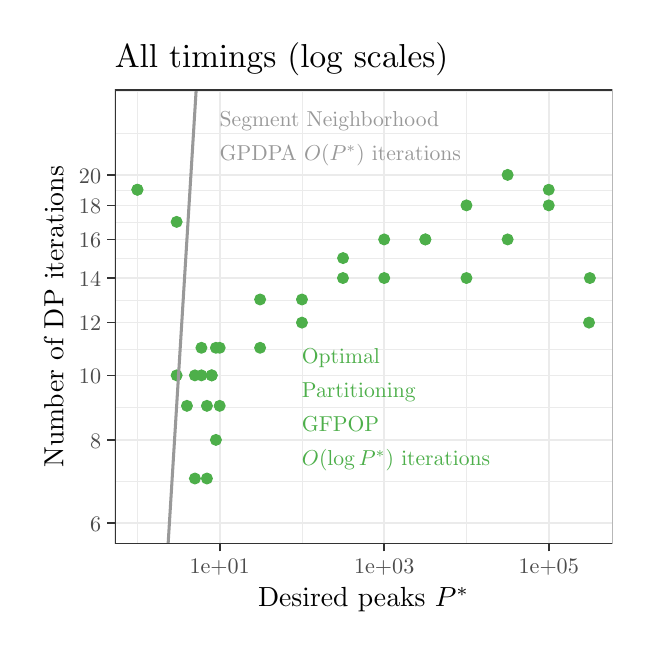
\begin{tikzpicture}[x=1pt,y=1pt]
\definecolor{fillColor}{RGB}{255,255,255}
\path[use as bounding box,fill=fillColor,fill opacity=0.00] (0,0) rectangle (216.81,216.81);
\begin{scope}
\path[clip] (  0.00,  0.00) rectangle (216.81,216.81);
\definecolor{drawColor}{RGB}{255,255,255}
\definecolor{fillColor}{RGB}{255,255,255}

\path[draw=drawColor,line width= 0.6pt,line join=round,line cap=round,fill=fillColor] (  0.00,  0.00) rectangle (216.81,216.81);
\end{scope}
\begin{scope}
\path[clip] ( 31.48, 30.33) rectangle (211.31,194.39);
\definecolor{fillColor}{RGB}{255,255,255}

\path[fill=fillColor] ( 31.48, 30.33) rectangle (211.31,194.39);
\definecolor{drawColor}{gray}{0.92}

\path[draw=drawColor,line width= 0.3pt,line join=round] ( 31.48, 52.82) --
	(211.31, 52.82);

\path[draw=drawColor,line width= 0.3pt,line join=round] ( 31.48, 79.51) --
	(211.31, 79.51);

\path[draw=drawColor,line width= 0.3pt,line join=round] ( 31.48,100.70) --
	(211.31,100.70);

\path[draw=drawColor,line width= 0.3pt,line join=round] ( 31.48,118.28) --
	(211.31,118.28);

\path[draw=drawColor,line width= 0.3pt,line join=round] ( 31.48,133.31) --
	(211.31,133.31);

\path[draw=drawColor,line width= 0.3pt,line join=round] ( 31.48,146.45) --
	(211.31,146.45);

\path[draw=drawColor,line width= 0.3pt,line join=round] ( 31.48,158.11) --
	(211.31,158.11);

\path[draw=drawColor,line width= 0.3pt,line join=round] ( 31.48,178.65) --
	(211.31,178.65);

\path[draw=drawColor,line width= 0.3pt,line join=round] ( 31.48,193.68) --
	(211.31,193.68);

\path[draw=drawColor,line width= 0.3pt,line join=round] ( 39.65, 30.33) --
	( 39.65,194.39);

\path[draw=drawColor,line width= 0.3pt,line join=round] ( 99.11, 30.33) --
	( 99.11,194.39);

\path[draw=drawColor,line width= 0.3pt,line join=round] (158.56, 30.33) --
	(158.56,194.39);

\path[draw=drawColor,line width= 0.6pt,line join=round] ( 31.48, 37.79) --
	(211.31, 37.79);

\path[draw=drawColor,line width= 0.6pt,line join=round] ( 31.48, 67.85) --
	(211.31, 67.85);

\path[draw=drawColor,line width= 0.6pt,line join=round] ( 31.48, 91.17) --
	(211.31, 91.17);

\path[draw=drawColor,line width= 0.6pt,line join=round] ( 31.48,110.23) --
	(211.31,110.23);

\path[draw=drawColor,line width= 0.6pt,line join=round] ( 31.48,126.34) --
	(211.31,126.34);

\path[draw=drawColor,line width= 0.6pt,line join=round] ( 31.48,140.29) --
	(211.31,140.29);

\path[draw=drawColor,line width= 0.6pt,line join=round] ( 31.48,152.60) --
	(211.31,152.60);

\path[draw=drawColor,line width= 0.6pt,line join=round] ( 31.48,163.61) --
	(211.31,163.61);

\path[draw=drawColor,line width= 0.6pt,line join=round] ( 69.38, 30.33) --
	( 69.38,194.39);

\path[draw=drawColor,line width= 0.6pt,line join=round] (128.84, 30.33) --
	(128.84,194.39);

\path[draw=drawColor,line width= 0.6pt,line join=round] (188.29, 30.33) --
	(188.29,194.39);
\definecolor{drawColor}{RGB}{77,175,74}
\definecolor{fillColor}{RGB}{77,175,74}

\path[draw=drawColor,line width= 0.4pt,line join=round,line cap=round,fill=fillColor] ( 39.65,158.25) circle (  1.96);

\path[draw=drawColor,line width= 0.4pt,line join=round,line cap=round,fill=fillColor] ( 53.83, 91.17) circle (  1.96);

\path[draw=drawColor,line width= 0.4pt,line join=round,line cap=round,fill=fillColor] ( 57.55, 80.16) circle (  1.96);

\path[draw=drawColor,line width= 0.4pt,line join=round,line cap=round,fill=fillColor] ( 60.43, 91.17) circle (  1.96);

\path[draw=drawColor,line width= 0.4pt,line join=round,line cap=round,fill=fillColor] ( 62.78,101.13) circle (  1.96);

\path[draw=drawColor,line width= 0.4pt,line join=round,line cap=round,fill=fillColor] ( 64.77, 53.90) circle (  1.96);

\path[draw=drawColor,line width= 0.4pt,line join=round,line cap=round,fill=fillColor] ( 66.50, 91.17) circle (  1.96);

\path[draw=drawColor,line width= 0.4pt,line join=round,line cap=round,fill=fillColor] ( 68.02,101.13) circle (  1.96);

\path[draw=drawColor,line width= 0.4pt,line join=round,line cap=round,fill=fillColor] ( 69.38, 80.16) circle (  1.96);

\path[draw=drawColor,line width= 0.4pt,line join=round,line cap=round,fill=fillColor] ( 83.99,118.59) circle (  1.96);

\path[draw=drawColor,line width= 0.4pt,line join=round,line cap=round,fill=fillColor] ( 99.11,110.23) circle (  1.96);

\path[draw=drawColor,line width= 0.4pt,line join=round,line cap=round,fill=fillColor] (113.96,133.55) circle (  1.96);

\path[draw=drawColor,line width= 0.4pt,line join=round,line cap=round,fill=fillColor] (128.82,140.29) circle (  1.96);

\path[draw=drawColor,line width= 0.4pt,line join=round,line cap=round,fill=fillColor] (143.70,140.29) circle (  1.96);

\path[draw=drawColor,line width= 0.4pt,line join=round,line cap=round,fill=fillColor] (158.56,152.60) circle (  1.96);

\path[draw=drawColor,line width= 0.4pt,line join=round,line cap=round,fill=fillColor] (173.43,163.61) circle (  1.96);

\path[draw=drawColor,line width= 0.4pt,line join=round,line cap=round,fill=fillColor] (188.29,152.60) circle (  1.96);

\path[draw=drawColor,line width= 0.4pt,line join=round,line cap=round,fill=fillColor] (203.14,126.34) circle (  1.96);

\path[draw=drawColor,line width= 0.4pt,line join=round,line cap=round,fill=fillColor] ( 39.65,158.25) circle (  1.96);

\path[draw=drawColor,line width= 0.4pt,line join=round,line cap=round,fill=fillColor] ( 53.83,146.63) circle (  1.96);

\path[draw=drawColor,line width= 0.4pt,line join=round,line cap=round,fill=fillColor] ( 60.43, 53.90) circle (  1.96);

\path[draw=drawColor,line width= 0.4pt,line join=round,line cap=round,fill=fillColor] ( 62.78, 91.17) circle (  1.96);

\path[draw=drawColor,line width= 0.4pt,line join=round,line cap=round,fill=fillColor] ( 64.77, 80.16) circle (  1.96);

\path[draw=drawColor,line width= 0.4pt,line join=round,line cap=round,fill=fillColor] ( 66.50, 91.17) circle (  1.96);

\path[draw=drawColor,line width= 0.4pt,line join=round,line cap=round,fill=fillColor] ( 68.02, 67.85) circle (  1.96);

\path[draw=drawColor,line width= 0.4pt,line join=round,line cap=round,fill=fillColor] ( 69.38,101.13) circle (  1.96);

\path[draw=drawColor,line width= 0.4pt,line join=round,line cap=round,fill=fillColor] ( 83.99,101.13) circle (  1.96);

\path[draw=drawColor,line width= 0.4pt,line join=round,line cap=round,fill=fillColor] ( 99.11,118.59) circle (  1.96);

\path[draw=drawColor,line width= 0.4pt,line join=round,line cap=round,fill=fillColor] (113.92,126.34) circle (  1.96);

\path[draw=drawColor,line width= 0.4pt,line join=round,line cap=round,fill=fillColor] (128.84,126.34) circle (  1.96);

\path[draw=drawColor,line width= 0.4pt,line join=round,line cap=round,fill=fillColor] (143.70,140.29) circle (  1.96);

\path[draw=drawColor,line width= 0.4pt,line join=round,line cap=round,fill=fillColor] (158.56,126.34) circle (  1.96);

\path[draw=drawColor,line width= 0.4pt,line join=round,line cap=round,fill=fillColor] (173.43,140.29) circle (  1.96);

\path[draw=drawColor,line width= 0.4pt,line join=round,line cap=round,fill=fillColor] (188.29,158.25) circle (  1.96);

\path[draw=drawColor,line width= 0.4pt,line join=round,line cap=round,fill=fillColor] (202.84,110.23) circle (  1.96);
\definecolor{drawColor}{gray}{0.60}

\path[draw=drawColor,line width= 1.1pt,line join=round] ( 48.88,  0.00) -- ( 62.27,216.81);

\node[text=drawColor,anchor=base west,inner sep=0pt, outer sep=0pt, scale=  0.78] at ( 69.38,181.20) {Segment Neighborhood};

\node[text=drawColor,anchor=base west,inner sep=0pt, outer sep=0pt, scale=  0.78] at ( 69.38,168.91) {GPDPA $O(P^*)$ iterations};

\node[text=drawColor,anchor=base west,inner sep=0pt, outer sep=0pt, scale=  0.78] at ( 69.38,156.62) {};

\node[text=drawColor,anchor=base west,inner sep=0pt, outer sep=0pt, scale=  0.78] at ( 69.38,144.32) {};
\definecolor{drawColor}{RGB}{77,175,74}

\node[text=drawColor,anchor=base west,inner sep=0pt, outer sep=0pt, scale=  0.78] at ( 99.11, 95.40) {Optimal};

\node[text=drawColor,anchor=base west,inner sep=0pt, outer sep=0pt, scale=  0.78] at ( 99.11, 83.11) {Partitioning};

\node[text=drawColor,anchor=base west,inner sep=0pt, outer sep=0pt, scale=  0.78] at ( 99.11, 70.81) {GFPOP};

\node[text=drawColor,anchor=base west,inner sep=0pt, outer sep=0pt, scale=  0.78] at ( 99.11, 58.52) {$O(\log P^*)$ iterations};
\definecolor{drawColor}{gray}{0.20}

\path[draw=drawColor,line width= 0.6pt,line join=round,line cap=round] ( 31.48, 30.33) rectangle (211.31,194.39);
\end{scope}
\begin{scope}
\path[clip] (  0.00,  0.00) rectangle (216.81,216.81);
\definecolor{drawColor}{gray}{0.30}

\node[text=drawColor,anchor=base east,inner sep=0pt, outer sep=0pt, scale=  0.80] at ( 26.53, 34.83) {6};

\node[text=drawColor,anchor=base east,inner sep=0pt, outer sep=0pt, scale=  0.80] at ( 26.53, 64.89) {8};

\node[text=drawColor,anchor=base east,inner sep=0pt, outer sep=0pt, scale=  0.80] at ( 26.53, 88.22) {10};

\node[text=drawColor,anchor=base east,inner sep=0pt, outer sep=0pt, scale=  0.80] at ( 26.53,107.27) {12};

\node[text=drawColor,anchor=base east,inner sep=0pt, outer sep=0pt, scale=  0.80] at ( 26.53,123.38) {14};

\node[text=drawColor,anchor=base east,inner sep=0pt, outer sep=0pt, scale=  0.80] at ( 26.53,137.34) {16};

\node[text=drawColor,anchor=base east,inner sep=0pt, outer sep=0pt, scale=  0.80] at ( 26.53,149.65) {18};

\node[text=drawColor,anchor=base east,inner sep=0pt, outer sep=0pt, scale=  0.80] at ( 26.53,160.66) {20};
\end{scope}
\begin{scope}
\path[clip] (  0.00,  0.00) rectangle (216.81,216.81);
\definecolor{drawColor}{gray}{0.20}

\path[draw=drawColor,line width= 0.6pt,line join=round] ( 28.73, 37.79) --
	( 31.48, 37.79);

\path[draw=drawColor,line width= 0.6pt,line join=round] ( 28.73, 67.85) --
	( 31.48, 67.85);

\path[draw=drawColor,line width= 0.6pt,line join=round] ( 28.73, 91.17) --
	( 31.48, 91.17);

\path[draw=drawColor,line width= 0.6pt,line join=round] ( 28.73,110.23) --
	( 31.48,110.23);

\path[draw=drawColor,line width= 0.6pt,line join=round] ( 28.73,126.34) --
	( 31.48,126.34);

\path[draw=drawColor,line width= 0.6pt,line join=round] ( 28.73,140.29) --
	( 31.48,140.29);

\path[draw=drawColor,line width= 0.6pt,line join=round] ( 28.73,152.60) --
	( 31.48,152.60);

\path[draw=drawColor,line width= 0.6pt,line join=round] ( 28.73,163.61) --
	( 31.48,163.61);
\end{scope}
\begin{scope}
\path[clip] (  0.00,  0.00) rectangle (216.81,216.81);
\definecolor{drawColor}{gray}{0.20}

\path[draw=drawColor,line width= 0.6pt,line join=round] ( 69.38, 27.58) --
	( 69.38, 30.33);

\path[draw=drawColor,line width= 0.6pt,line join=round] (128.84, 27.58) --
	(128.84, 30.33);

\path[draw=drawColor,line width= 0.6pt,line join=round] (188.29, 27.58) --
	(188.29, 30.33);
\end{scope}
\begin{scope}
\path[clip] (  0.00,  0.00) rectangle (216.81,216.81);
\definecolor{drawColor}{gray}{0.30}

\node[text=drawColor,anchor=base,inner sep=0pt, outer sep=0pt, scale=  0.80] at ( 69.38, 19.46) {1e+01};

\node[text=drawColor,anchor=base,inner sep=0pt, outer sep=0pt, scale=  0.80] at (128.84, 19.46) {1e+03};

\node[text=drawColor,anchor=base,inner sep=0pt, outer sep=0pt, scale=  0.80] at (188.29, 19.46) {1e+05};
\end{scope}
\begin{scope}
\path[clip] (  0.00,  0.00) rectangle (216.81,216.81);
\definecolor{drawColor}{RGB}{0,0,0}

\node[text=drawColor,anchor=base,inner sep=0pt, outer sep=0pt, scale=  1.00] at (121.39,  7.62) {Desired peaks $P^*$};
\end{scope}
\begin{scope}
\path[clip] (  0.00,  0.00) rectangle (216.81,216.81);
\definecolor{drawColor}{RGB}{0,0,0}

\node[text=drawColor,rotate= 90.00,anchor=base,inner sep=0pt, outer sep=0pt, scale=  1.00] at ( 12.89,112.36) {Number of DP iterations};
\end{scope}
\begin{scope}
\path[clip] (  0.00,  0.00) rectangle (216.81,216.81);
\definecolor{drawColor}{RGB}{0,0,0}

\node[text=drawColor,anchor=base west,inner sep=0pt, outer sep=0pt, scale=  1.20] at ( 31.48,202.44) {All timings (log scales)};
\end{scope}
\end{tikzpicture}

\end{minipage}
\begin{minipage}{3in} 
  % Created by tikzDevice version 0.12.3 on 2020-01-08 13:37:48
% !TEX encoding = UTF-8 Unicode
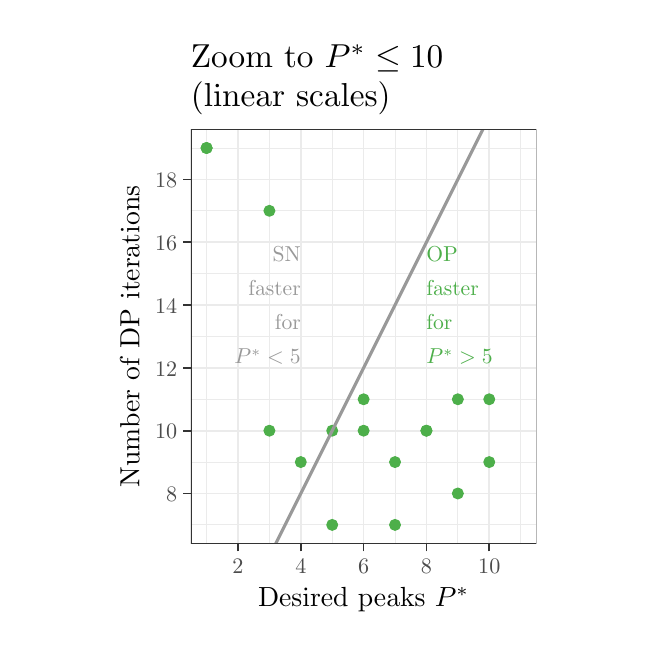
\begin{tikzpicture}[x=1pt,y=1pt]
\definecolor{fillColor}{RGB}{255,255,255}
\path[use as bounding box,fill=fillColor,fill opacity=0.00] (0,0) rectangle (216.81,216.81);
\begin{scope}
\path[clip] ( 27.50,  0.00) rectangle (189.31,216.81);
\definecolor{drawColor}{RGB}{255,255,255}
\definecolor{fillColor}{RGB}{255,255,255}

\path[draw=drawColor,line width= 0.6pt,line join=round,line cap=round,fill=fillColor] ( 27.50,  0.00) rectangle (189.31,216.81);
\end{scope}
\begin{scope}
\path[clip] ( 58.97, 30.33) rectangle (183.81,180.14);
\definecolor{fillColor}{RGB}{255,255,255}

\path[fill=fillColor] ( 58.97, 30.33) rectangle (183.81,180.14);
\definecolor{drawColor}{gray}{0.92}

\path[draw=drawColor,line width= 0.3pt,line join=round] ( 58.97, 37.14) --
	(183.81, 37.14);

\path[draw=drawColor,line width= 0.3pt,line join=round] ( 58.97, 59.84) --
	(183.81, 59.84);

\path[draw=drawColor,line width= 0.3pt,line join=round] ( 58.97, 82.53) --
	(183.81, 82.53);

\path[draw=drawColor,line width= 0.3pt,line join=round] ( 58.97,105.23) --
	(183.81,105.23);

\path[draw=drawColor,line width= 0.3pt,line join=round] ( 58.97,127.93) --
	(183.81,127.93);

\path[draw=drawColor,line width= 0.3pt,line join=round] ( 58.97,150.63) --
	(183.81,150.63);

\path[draw=drawColor,line width= 0.3pt,line join=round] ( 58.97,173.33) --
	(183.81,173.33);

\path[draw=drawColor,line width= 0.3pt,line join=round] ( 64.65, 30.33) --
	( 64.65,180.14);

\path[draw=drawColor,line width= 0.3pt,line join=round] ( 87.35, 30.33) --
	( 87.35,180.14);

\path[draw=drawColor,line width= 0.3pt,line join=round] (110.04, 30.33) --
	(110.04,180.14);

\path[draw=drawColor,line width= 0.3pt,line join=round] (132.74, 30.33) --
	(132.74,180.14);

\path[draw=drawColor,line width= 0.3pt,line join=round] (155.44, 30.33) --
	(155.44,180.14);

\path[draw=drawColor,line width= 0.3pt,line join=round] (178.14, 30.33) --
	(178.14,180.14);

\path[draw=drawColor,line width= 0.6pt,line join=round] ( 58.97, 48.49) --
	(183.81, 48.49);

\path[draw=drawColor,line width= 0.6pt,line join=round] ( 58.97, 71.18) --
	(183.81, 71.18);

\path[draw=drawColor,line width= 0.6pt,line join=round] ( 58.97, 93.88) --
	(183.81, 93.88);

\path[draw=drawColor,line width= 0.6pt,line join=round] ( 58.97,116.58) --
	(183.81,116.58);

\path[draw=drawColor,line width= 0.6pt,line join=round] ( 58.97,139.28) --
	(183.81,139.28);

\path[draw=drawColor,line width= 0.6pt,line join=round] ( 58.97,161.98) --
	(183.81,161.98);

\path[draw=drawColor,line width= 0.6pt,line join=round] ( 76.00, 30.33) --
	( 76.00,180.14);

\path[draw=drawColor,line width= 0.6pt,line join=round] ( 98.69, 30.33) --
	( 98.69,180.14);

\path[draw=drawColor,line width= 0.6pt,line join=round] (121.39, 30.33) --
	(121.39,180.14);

\path[draw=drawColor,line width= 0.6pt,line join=round] (144.09, 30.33) --
	(144.09,180.14);

\path[draw=drawColor,line width= 0.6pt,line join=round] (166.79, 30.33) --
	(166.79,180.14);
\definecolor{drawColor}{RGB}{77,175,74}
\definecolor{fillColor}{RGB}{77,175,74}

\path[draw=drawColor,line width= 0.4pt,line join=round,line cap=round,fill=fillColor] ( 64.65,173.33) circle (  1.96);

\path[draw=drawColor,line width= 0.4pt,line join=round,line cap=round,fill=fillColor] ( 87.35, 71.18) circle (  1.96);

\path[draw=drawColor,line width= 0.4pt,line join=round,line cap=round,fill=fillColor] ( 98.69, 59.84) circle (  1.96);

\path[draw=drawColor,line width= 0.4pt,line join=round,line cap=round,fill=fillColor] (110.04, 71.18) circle (  1.96);

\path[draw=drawColor,line width= 0.4pt,line join=round,line cap=round,fill=fillColor] (121.39, 82.53) circle (  1.96);

\path[draw=drawColor,line width= 0.4pt,line join=round,line cap=round,fill=fillColor] (132.74, 37.14) circle (  1.96);

\path[draw=drawColor,line width= 0.4pt,line join=round,line cap=round,fill=fillColor] (144.09, 71.18) circle (  1.96);

\path[draw=drawColor,line width= 0.4pt,line join=round,line cap=round,fill=fillColor] (155.44, 82.53) circle (  1.96);

\path[draw=drawColor,line width= 0.4pt,line join=round,line cap=round,fill=fillColor] (166.79, 59.84) circle (  1.96);

\path[draw=drawColor,line width= 0.4pt,line join=round,line cap=round,fill=fillColor] ( 64.65,173.33) circle (  1.96);

\path[draw=drawColor,line width= 0.4pt,line join=round,line cap=round,fill=fillColor] ( 87.35,150.63) circle (  1.96);

\path[draw=drawColor,line width= 0.4pt,line join=round,line cap=round,fill=fillColor] (110.04, 37.14) circle (  1.96);

\path[draw=drawColor,line width= 0.4pt,line join=round,line cap=round,fill=fillColor] (121.39, 71.18) circle (  1.96);

\path[draw=drawColor,line width= 0.4pt,line join=round,line cap=round,fill=fillColor] (132.74, 59.84) circle (  1.96);

\path[draw=drawColor,line width= 0.4pt,line join=round,line cap=round,fill=fillColor] (144.09, 71.18) circle (  1.96);

\path[draw=drawColor,line width= 0.4pt,line join=round,line cap=round,fill=fillColor] (155.44, 48.49) circle (  1.96);

\path[draw=drawColor,line width= 0.4pt,line join=round,line cap=round,fill=fillColor] (166.79, 82.53) circle (  1.96);
\definecolor{drawColor}{gray}{0.60}

\path[draw=drawColor,line width= 1.1pt,line join=round] ( 74.45,  0.00) -- (182.86,216.81);

\node[text=drawColor,anchor=base east,inner sep=0pt, outer sep=0pt, scale=  0.78] at ( 98.69,132.15) {SN};

\node[text=drawColor,anchor=base east,inner sep=0pt, outer sep=0pt, scale=  0.78] at ( 98.69,119.86) {faster};

\node[text=drawColor,anchor=base east,inner sep=0pt, outer sep=0pt, scale=  0.78] at ( 98.69,107.57) {for};

\node[text=drawColor,anchor=base east,inner sep=0pt, outer sep=0pt, scale=  0.78] at ( 98.69, 95.28) {$P^*<5$};
\definecolor{drawColor}{RGB}{77,175,74}

\node[text=drawColor,anchor=base west,inner sep=0pt, outer sep=0pt, scale=  0.78] at (144.09,132.15) {OP};

\node[text=drawColor,anchor=base west,inner sep=0pt, outer sep=0pt, scale=  0.78] at (144.09,119.86) {faster};

\node[text=drawColor,anchor=base west,inner sep=0pt, outer sep=0pt, scale=  0.78] at (144.09,107.57) {for};

\node[text=drawColor,anchor=base west,inner sep=0pt, outer sep=0pt, scale=  0.78] at (144.09, 95.28) {$P^*>5$};
\definecolor{drawColor}{gray}{0.20}

\path[draw=drawColor,line width= 0.6pt,line join=round,line cap=round] ( 58.97, 30.33) rectangle (183.81,180.14);
\end{scope}
\begin{scope}
\path[clip] (  0.00,  0.00) rectangle (216.81,216.81);
\definecolor{drawColor}{gray}{0.30}

\node[text=drawColor,anchor=base east,inner sep=0pt, outer sep=0pt, scale=  0.80] at ( 54.02, 45.53) {8};

\node[text=drawColor,anchor=base east,inner sep=0pt, outer sep=0pt, scale=  0.80] at ( 54.02, 68.23) {10};

\node[text=drawColor,anchor=base east,inner sep=0pt, outer sep=0pt, scale=  0.80] at ( 54.02, 90.93) {12};

\node[text=drawColor,anchor=base east,inner sep=0pt, outer sep=0pt, scale=  0.80] at ( 54.02,113.62) {14};

\node[text=drawColor,anchor=base east,inner sep=0pt, outer sep=0pt, scale=  0.80] at ( 54.02,136.32) {16};

\node[text=drawColor,anchor=base east,inner sep=0pt, outer sep=0pt, scale=  0.80] at ( 54.02,159.02) {18};
\end{scope}
\begin{scope}
\path[clip] (  0.00,  0.00) rectangle (216.81,216.81);
\definecolor{drawColor}{gray}{0.20}

\path[draw=drawColor,line width= 0.6pt,line join=round] ( 56.22, 48.49) --
	( 58.97, 48.49);

\path[draw=drawColor,line width= 0.6pt,line join=round] ( 56.22, 71.18) --
	( 58.97, 71.18);

\path[draw=drawColor,line width= 0.6pt,line join=round] ( 56.22, 93.88) --
	( 58.97, 93.88);

\path[draw=drawColor,line width= 0.6pt,line join=round] ( 56.22,116.58) --
	( 58.97,116.58);

\path[draw=drawColor,line width= 0.6pt,line join=round] ( 56.22,139.28) --
	( 58.97,139.28);

\path[draw=drawColor,line width= 0.6pt,line join=round] ( 56.22,161.98) --
	( 58.97,161.98);
\end{scope}
\begin{scope}
\path[clip] (  0.00,  0.00) rectangle (216.81,216.81);
\definecolor{drawColor}{gray}{0.20}

\path[draw=drawColor,line width= 0.6pt,line join=round] ( 76.00, 27.58) --
	( 76.00, 30.33);

\path[draw=drawColor,line width= 0.6pt,line join=round] ( 98.69, 27.58) --
	( 98.69, 30.33);

\path[draw=drawColor,line width= 0.6pt,line join=round] (121.39, 27.58) --
	(121.39, 30.33);

\path[draw=drawColor,line width= 0.6pt,line join=round] (144.09, 27.58) --
	(144.09, 30.33);

\path[draw=drawColor,line width= 0.6pt,line join=round] (166.79, 27.58) --
	(166.79, 30.33);
\end{scope}
\begin{scope}
\path[clip] (  0.00,  0.00) rectangle (216.81,216.81);
\definecolor{drawColor}{gray}{0.30}

\node[text=drawColor,anchor=base,inner sep=0pt, outer sep=0pt, scale=  0.80] at ( 76.00, 19.46) {2};

\node[text=drawColor,anchor=base,inner sep=0pt, outer sep=0pt, scale=  0.80] at ( 98.69, 19.46) {4};

\node[text=drawColor,anchor=base,inner sep=0pt, outer sep=0pt, scale=  0.80] at (121.39, 19.46) {6};

\node[text=drawColor,anchor=base,inner sep=0pt, outer sep=0pt, scale=  0.80] at (144.09, 19.46) {8};

\node[text=drawColor,anchor=base,inner sep=0pt, outer sep=0pt, scale=  0.80] at (166.79, 19.46) {10};
\end{scope}
\begin{scope}
\path[clip] (  0.00,  0.00) rectangle (216.81,216.81);
\definecolor{drawColor}{RGB}{0,0,0}

\node[text=drawColor,anchor=base,inner sep=0pt, outer sep=0pt, scale=  1.00] at (121.39,  7.62) {Desired peaks $P^*$};
\end{scope}
\begin{scope}
\path[clip] (  0.00,  0.00) rectangle (216.81,216.81);
\definecolor{drawColor}{RGB}{0,0,0}

\node[text=drawColor,rotate= 90.00,anchor=base,inner sep=0pt, outer sep=0pt, scale=  1.00] at ( 40.39,105.23) {Number of DP iterations};
\end{scope}
\begin{scope}
\path[clip] (  0.00,  0.00) rectangle (216.81,216.81);
\definecolor{drawColor}{RGB}{0,0,0}

\node[text=drawColor,anchor=base west,inner sep=0pt, outer sep=0pt, scale=  1.20] at ( 58.97,202.44) {Zoom to $P^* \leq 10$};

\node[text=drawColor,anchor=base west,inner sep=0pt, outer sep=0pt, scale=  1.20] at ( 58.97,188.18) {(linear scales)};
\end{scope}
\end{tikzpicture}

\end{minipage}
\vskip -0.5cm
\caption{\label{fig:variable-peaks} Comparison of iterations using
  Segment Neighborhood (grey lines) and Optimal Partitioning (green
  dots). GFPOP with sequential search
  (Algorithm~\ref{algo:seq-search}) was used to compute optimal models
  with different numbers of peaks $P$, for two data sets with
  $N\approx 6\times 10^5$. \textbf{Left:} the number of iterations is
  linear $O(P)$ for Segment Neighborhood (grey lines) but empirically
  $O(\log P)$ for Optimal Partitioning with sequential search (green
  dots). \textbf{Right:} Optimal Partitioning is empirically faster
  for computing models with $P>5$ peaks (10 segments); Segment
  Neighborhood is faster for smaller models.}
\end{figure}



 

% \begin{CodeChunk}
% \begin{CodeInput}
% R> m_pois <- glm(Days ~ (Eth + Sex + Age + Lrn)^2, data = quine,
% +    family = poisson)
% \end{CodeInput}
% \end{CodeChunk}
% %
% To account for potential overdispersion we also consider a negative binomial
% GLM.
% %
% \begin{CodeChunk}
% \begin{CodeInput}
% R> library("MASS")
% R> m_nbin <- glm.nb(Days ~ (Eth + Sex + Age + Lrn)^2, data = quine)
% \end{CodeInput}
% \end{CodeChunk}
% %
% In a comparison with the BIC the latter model is clearly preferred.
% %
% \begin{CodeChunk}
% \begin{CodeInput}
% R> BIC(m_pois, m_nbin)
% \end{CodeInput}
% \begin{CodeOutput}
%        df      BIC
% m_pois 18 2046.851
% m_nbin 19 1157.235
% \end{CodeOutput}
% \end{CodeChunk}
% %
% Hence, the full summary of that model is shown below.
% %
% \begin{CodeChunk}
% \begin{CodeInput}
% R> summary(m_nbin)
% \end{CodeInput}
% \begin{CodeOutput}
% Call:
% glm.nb(formula = Days ~ (Eth + Sex + Age + Lrn)^2, data = quine, 
%     init.theta = 1.60364105, link = log)

% Deviance Residuals: 
%     Min       1Q   Median       3Q      Max  
% -3.0857  -0.8306  -0.2620   0.4282   2.0898  

% Coefficients: (1 not defined because of singularities)
%             Estimate Std. Error z value Pr(>|z|)    
% (Intercept)  3.00155    0.33709   8.904  < 2e-16 ***
% EthN        -0.24591    0.39135  -0.628  0.52977    
% SexM        -0.77181    0.38021  -2.030  0.04236 *  
% AgeF1       -0.02546    0.41615  -0.061  0.95121    
% AgeF2       -0.54884    0.54393  -1.009  0.31296    
% AgeF3       -0.25735    0.40558  -0.635  0.52574    
% LrnSL        0.38919    0.48421   0.804  0.42153    
% EthN:SexM    0.36240    0.29430   1.231  0.21818    
% EthN:AgeF1  -0.70000    0.43646  -1.604  0.10876    
% EthN:AgeF2  -1.23283    0.42962  -2.870  0.00411 ** 
% EthN:AgeF3   0.04721    0.44883   0.105  0.91622    
% EthN:LrnSL   0.06847    0.34040   0.201  0.84059    
% SexM:AgeF1   0.02257    0.47360   0.048  0.96198    
% SexM:AgeF2   1.55330    0.51325   3.026  0.00247 ** 
% SexM:AgeF3   1.25227    0.45539   2.750  0.00596 ** 
% SexM:LrnSL   0.07187    0.40805   0.176  0.86019    
% AgeF1:LrnSL -0.43101    0.47948  -0.899  0.36870    
% AgeF2:LrnSL  0.52074    0.48567   1.072  0.28363    
% AgeF3:LrnSL       NA         NA      NA       NA    
% ---
% Signif. codes:  0 '***' 0.001 '**' 0.01 '*' 0.05 '.' 0.1 ' ' 1

% (Dispersion parameter for Negative Binomial(1.6036) family taken to be 1)

%     Null deviance: 235.23  on 145  degrees of freedom
% Residual deviance: 167.53  on 128  degrees of freedom
% AIC: 1100.5

% Number of Fisher Scoring iterations: 1


%               Theta:  1.604 
%           Std. Err.:  0.214 

%  2 x log-likelihood:  -1062.546 
% \end{CodeOutput}
% \end{CodeChunk}



%% -- Summary/conclusions/discussion -------------------------------------------

\section{Summary and discussion} \label{sec:summary}


%% -- Optional special unnumbered sections -------------------------------------

\section*{Computational details}

The pseudocode for the algorithm which implements the dynamic
programming updates (\ref{eq:generalDP}) is stated below.
\begin{algorithm}
\begin{algorithmic}[1]
\STATE Input: data $\mathbf y$ and weights $\mathbf w$ (both size $n$), 
number of vertices/states $|V|$, starts $\underline S\subseteq V$, 
edges/transitions $E$.
\STATE Allocate $|V|\times n$ array of optimal cost functions $C_{s,t}$, 
each initialized to NULL.
\STATE for $t$ from $1$ to $n$:
\begin{ALC@g}
  \STATE if $t==1$:
  \begin{ALC@g}
    \STATE for $s$ in $\underline S$: // initialize cost for all possible starting states
    \begin{ALC@g}
      \STATE $C_{s,t}\gets\text{InitialCost}(y_t, w_t)$
    \end{ALC@g}
  \end{ALC@g}
  \STATE else:
  \begin{ALC@g}
    \STATE for $s$ from $1$ to $|V|$: 
    \begin{ALC@g}
      \STATE if $C_{s,t-1}$ is NOT NULL: // previous cost in this state has been computed
      \begin{ALC@g}
        \STATE $C_{s,t}\gets C_{s,t-1}$ // cost of staying in this state (no change)
      \end{ALC@g}
    \end{ALC@g}
    \STATE for ($\underline v$, $\overline v$, $\lambda$,
    ConstrainedCost) in $E$:
    \begin{ALC@g}
      \STATE if $C_{\underline v,t-1}$ is NOT NULL: // previous cost has been computed
      \begin{ALC@g}
        \STATE
        $\text{cost\_of\_change}\gets
        \text{ConstrainedCost}(C_{\underline v, t-1})$
        \STATE
        $\text{cost\_of\_change.set}
        (\underline v, t-1)$
        \STATE
        $\text{cost\_of\_change.addPenalty}
        (\text{$\lambda$})$
        \STATE if $C_{\overline v,t}$ is NULL:
        \begin{ALC@g}
          \STATE $C_{\overline v,t}\gets\text{cost\_of\_change}$
        \end{ALC@g}
        \STATE else:
        \begin{ALC@g}
          \STATE
          $C_{\overline v,t}\gets \text{MinOfTwo}(C_{\overline v,t},
          \text{cost\_of\_change})$
        \end{ALC@g}
      \end{ALC@g}
    \end{ALC@g}
    \STATE for $s$ from $1$ to $|V|$:
    \begin{ALC@g}
      \STATE if $C_{s,t}$ is NOT NULL:
      \begin{ALC@g}
        \STATE $C_{s,t}\text{.addDataPoint}(y_t, w_t)$
      \end{ALC@g}
    \end{ALC@g}
  \end{ALC@g}
\end{ALC@g}
\STATE Output: $|V|\times n$ array of optimal cost functions $C_{s,t}$.
\caption{\label{algo:GFPOP}Generalized Functional Pruning Optimal
  Partitioning Algorithm, Dynamic Programming (GFPOP-DP)}
\end{algorithmic}
\end{algorithm}

The algorithm above performs several checks if $C_{s,t}$ is NULL or
not (lines 9, 12, 16, 21). All costs are initialized as NULL (line
2). After having performed the cost update for data $t$, a NULL cost
$C_{s,t}$ means that state $s$ is not feasible at data $t$. For each
constraint function $g$ there is a corresponding ConstrainedCost
sub-routine that is mentioned on lines~11 and 13 (e.g. no constraint
$g_0$ MinUnconstrained, non-decreasing change $g_\uparrow$ MinLess,
non-increasing change $g_\downarrow$ MinMore). 

The average time and space complexity of Algorithm~\ref{algo:GFPOP} is
$O(|V| n I)$ where $|V|$ is the number of states and $I$ is the
average number of of intervals stored in the $|V|\times n$ array of
$C_{s,t}$ cost functions. We observed that $I=\log n$ in the empirical
tests of the peak detection model on ChIP-seq data
(Section~\ref{sec:results_time}), so we expect that the average time
complexity of Algorithm~\ref{algo:GFPOP} is $O(|V| n\log n)$.

Note that the algorithm above only performs the dynamic
programming. The decoding of optimal model parameters is achieved
using the algorithm below.

\begin{algorithm}
\begin{algorithmic}[1]
\STATE Output: $|V|\times n$ array of optimal cost functions $C_{s,t}$, 
ends $\overline S\subseteq V$.
\STATE Allocate
$\mathbf m\in\RR^n$ (mean), 
$\mathbf s\in\ZZ^n$ (state), 
$\mathbf t\in\ZZ^n$ (segment end).  
\STATE $u^*,s^*,t',s'\gets \text{ArgMin}(C_{\cdot,n}, \overline S)$ // begin decoding
\STATE $i\gets 1;\, m_{i}\gets u^*;\, s_i\gets s^*;\, t_{i}\gets n$
\STATE while $t' > 0$:
\begin{ALC@g}
  \STATE $i\gets i+1;\, t_{i}\gets t'$
  \STATE $u^*,s^*,t',s'\gets \text{ArgMin}(C_{s',t'})$
  \STATE $m_{i}\gets u^*;\, s_i\gets s^*$
\end{ALC@g}
\STATE Output: 
$\mathbf m$, 
$\mathbf s$, 
$\mathbf t$.
\caption{\label{algo:GFPOP-decode}Generalized Functional Pruning Optimal
  Partitioning Algorithm, decoding (GFPOP-decode)}
\end{algorithmic}
\end{algorithm}


% \begin{leftbar} 
% If necessary or useful, information about certain computational details
% such as version numbers, operating systems, or compilers could be included
% in an unnumbered section. Also, auxiliary packages (say, for visualizations,
% maps, tables, \dots) that are not cited in the main text can be credited here.
% \end{leftbar}

% The results in this paper were obtained using
% \proglang{R}~3.4.1 with the
% \pkg{MASS}~7.3.47 package. \proglang{R} itself
% and all packages used are available from the Comprehensive
% \proglang{R} Archive Network (CRAN) at
% \url{https://CRAN.R-project.org/}.


\section*{Acknowledgments}

% \begin{leftbar}
% All acknowledgments (note the AE spelling) should be collected in this
% unnumbered section before the references. It may contain the usual information
% about funding and feedback from colleagues/reviewers/etc. Furthermore,
% information such as relative contributions of the authors may be added here
% (if any).
% \end{leftbar}


%% -- Bibliography -------------------------------------------------------------
%% - References need to be provided in a .bib BibTeX database.
%% - All references should be made with \cite, \citet, \citep, \citealp etc.
%%   (and never hard-coded). See the FAQ for details.
%% - JSS-specific markup (\proglang, \pkg, \code) should be used in the .bib.
%% - Titles in the .bib should be in title case.
%% - DOIs should be included where available.

\bibliography{jss-refs}


% %% -- Appendix (if any) --------------------------------------------------------
% %% - After the bibliography with page break.
% %% - With proper section titles and _not_ just "Appendix".

% \newpage

% \begin{appendix}

% \section{More technical details} \label{app:technical}

% \begin{leftbar}
% Appendices can be included after the bibliography (with a page break). Each
% section within the appendix should have a proper section title (rather than
% just \emph{Appendix}).

% For more technical style details, please check out JSS's style FAQ at
% \url{https://www.jstatsoft.org/pages/view/style#frequently-asked-questions}
% which includes the following topics:
% \begin{itemize}
%   \item Title vs.\ sentence case.
%   \item Graphics formatting.
%   \item Naming conventions.
%   \item Turning JSS manuscripts into \proglang{R} package vignettes.
%   \item Trouble shooting.
%   \item Many other potentially helpful details\dots
% \end{itemize}
% \end{leftbar}


% \section[Using BibTeX]{Using \textsc{Bib}{\TeX}} \label{app:bibtex}

% \begin{leftbar}
% References need to be provided in a \textsc{Bib}{\TeX} file (\code{.bib}). All
% references should be made with \verb|\cite|, \verb|\citet|, \verb|\citep|,
% \verb|\citealp| etc.\ (and never hard-coded). This commands yield different
% formats of author-year citations and allow to include additional details (e.g.,
% pages, chapters, \dots) in brackets. In case you are not familiar with these
% commands see the JSS style FAQ for details.

% Cleaning up \textsc{Bib}{\TeX} files is a somewhat tedious task -- especially
% when acquiring the entries automatically from mixed online sources. However,
% it is important that informations are complete and presented in a consistent
% style to avoid confusions. JSS requires the following format.
% \begin{itemize}
%   \item JSS-specific markup (\verb|\proglang|, \verb|\pkg|, \verb|\code|) should
%     be used in the references.
%   \item Titles should be in title case.
%   \item Journal titles should not be abbreviated and in title case.
%   \item DOIs should be included where available.
%   \item Software should be properly cited as well. For \proglang{R} packages
%     \code{citation("pkgname")} typically provides a good starting point.
% \end{itemize}
% \end{leftbar}

% \end{appendix}

% %% -----------------------------------------------------------------------------


\end{document}
